%%%%%%%%%%%%%%%%%%%%%%%%%%%%%%%%%%%%%%%%%%%%%%%%%%%%%%%%%%%%%%%%%%%%%%%%
%    INSTITUTE OF PHYSICS PUBLISHING                                   %
%                                                                      %
%   `Preparing an article for publication in an Institute of Physics   %
%    Publishing journal using LaTeX'                                   %
%                                                                      %
%    LaTeX source code `ioplau2e.tex' used to generate `author         %
%    guidelines', the documentation explaining and demonstrating use   %
%    of the Institute of Physics Publishing LaTeX preprint files       %
%    `iopart.cls, iopart12.clo and iopart10.clo'.                      %
%                                                                      %
%    `ioplau2e.tex' itself uses LaTeX with `iopart.cls'                %
%                                                                      %
%%%%%%%%%%%%%%%%%%%%%%%%%%%%%%%%%%
%
%
% First we have a character check
%
% ! exclamation mark    " double quote  
% # hash                ` opening quote (grave)
% & ampersand           ' closing quote (acute)
% $ dollar              % percent       
% ( open parenthesis    ) close paren.  
% - hyphen              = equals sign
% | vertical bar        ~ tilde         
% @ at sign             _ underscore
% { open curly brace    } close curly   
% [ open square         ] close square bracket
% + plus sign           ; semi-colon    
% * asterisk            : colon
% < open angle bracket  > close angle   
% , comma               . full stop
% ? question mark       / forward slash 
% \ backslash           ^ circumflex
%
% ABCDEFGHIJKLMNOPQRSTUVWXYZ 
% abcdefghijklmnopqrstuvwxyz 
% 1234567890
%
%%%%%%%%%%%%%%%%%%%%%%%%%%%%%%%%%%%%%%%%%%%%%%%%%%%%%%%%%%%%%%%%%%%
%
\documentclass[12pt]{iopart}
%\newcommand{\gguide}{{\it Preparing graphics for IOP Publishing journals}}
%Uncomment next line if AMS fonts required
\usepackage{iopams}  
\usepackage{epsfig}
\usepackage{verbatim}
\usepackage{hyperref}
\usepackage{harvard}
\usepackage{url}
%\usepackage{graphicx}
\begin{document}

\title[TwoSpect: Scorpius X-1]{TwoSpect: search for a simulated Scorpius X-1}

\author{Grant David Meadors$^1$, Evan Goetz$^2$, Keith Riles$^2$}

\address{$^1$Max-Planck-Institut f\"{u}r Gravitationsphysik, Am M\"{u}hlenberg 1, 14476 Potsdam and Callinstra{\ss}e 38, 30167 Hannover, Germany}
\address{$^2$University of Michigan, 450 Church Street, Ann Arbor, Michigan 48109, USA}
\ead{grant.meadors@aei.mpg.de}
\vspace{10pt}
%\begin{indented}
%\item[]February 2014
%\end{indented}
\date{\today}

\section{Technical notes}

\begin{figure}
\begin{center}
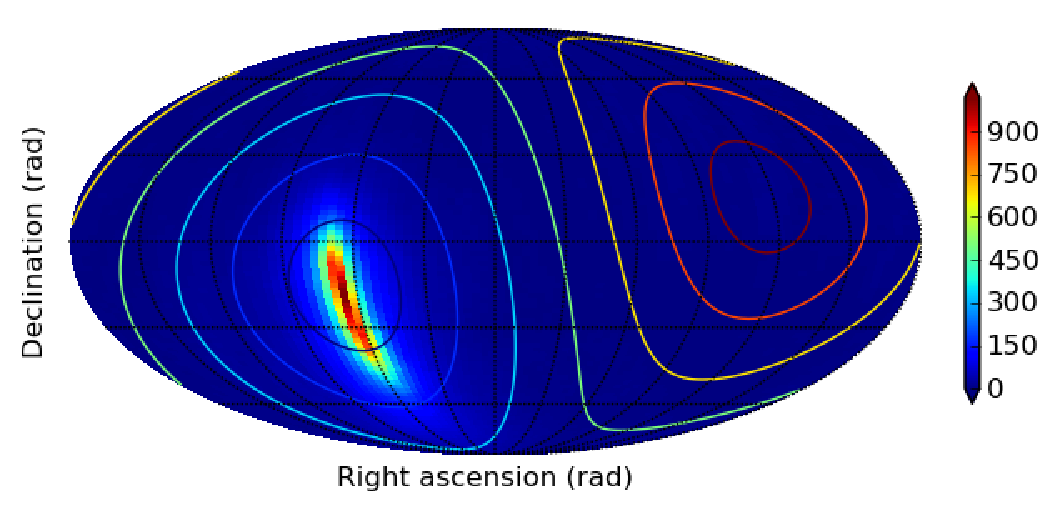
\includegraphics[width=0.6\paperwidth,height=0.2\paperheight]{plots/maptrueH1.eps}
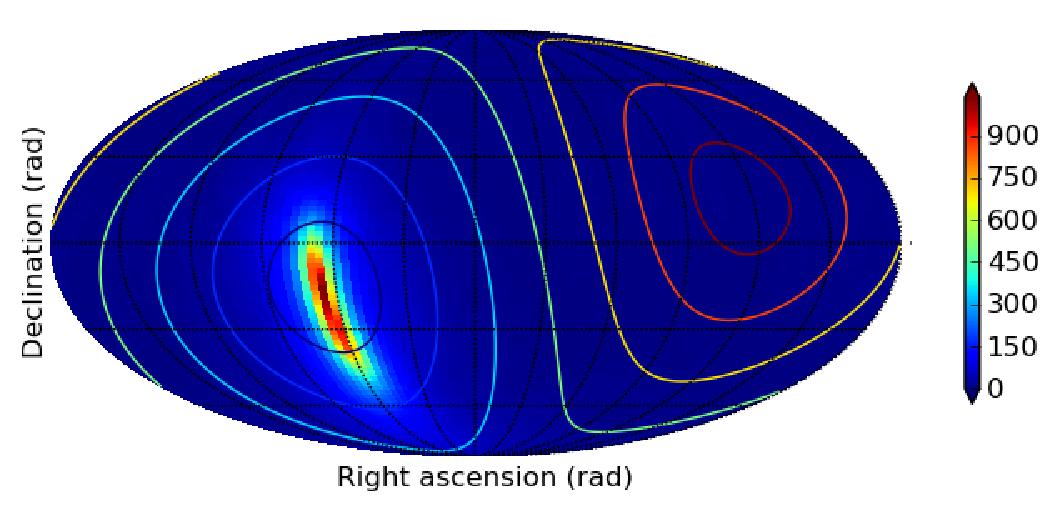
\includegraphics[width=0.6\paperwidth,height=0.2\paperheight]{plots/maptrueL1.eps}
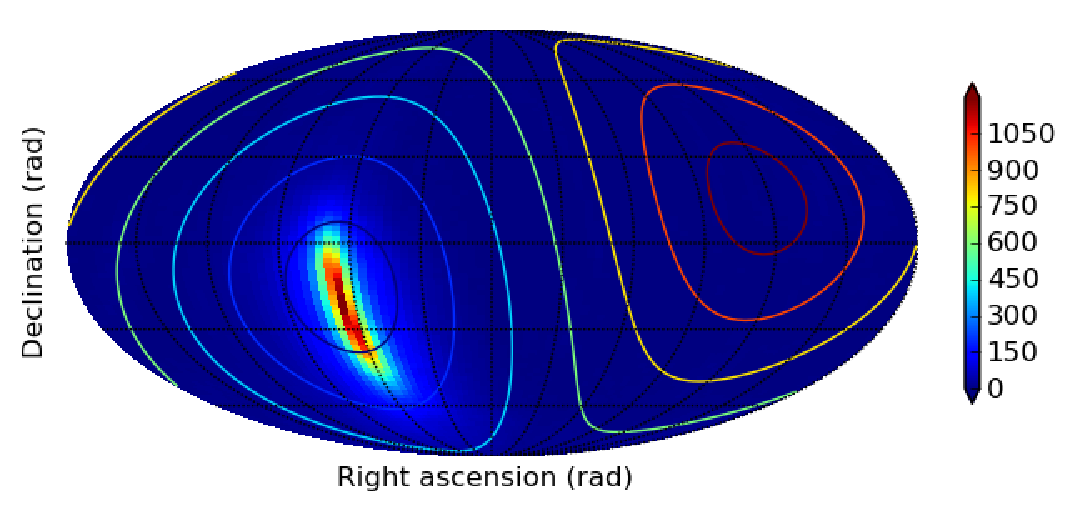
\includegraphics[width=0.6\paperwidth,height=0.2\paperheight]{plots/maptrueV1.eps}
\caption{ All-sky maps (from top to bottom: H1, L1, V1) showing analysis across varying right ascension and declination. 
Scorpius X-1 mock data challenge pulsar 16 (101x101 templates), showing $-\log_{10}p$-value on a Mollweide projection.
Contour lines at 1-radian great-circle distance intervals from the simulated location of Sco X-1.
}
\label{scox1-allsky-maps}
\end{center}
\end{figure}


\begin{figure}
\begin{center}
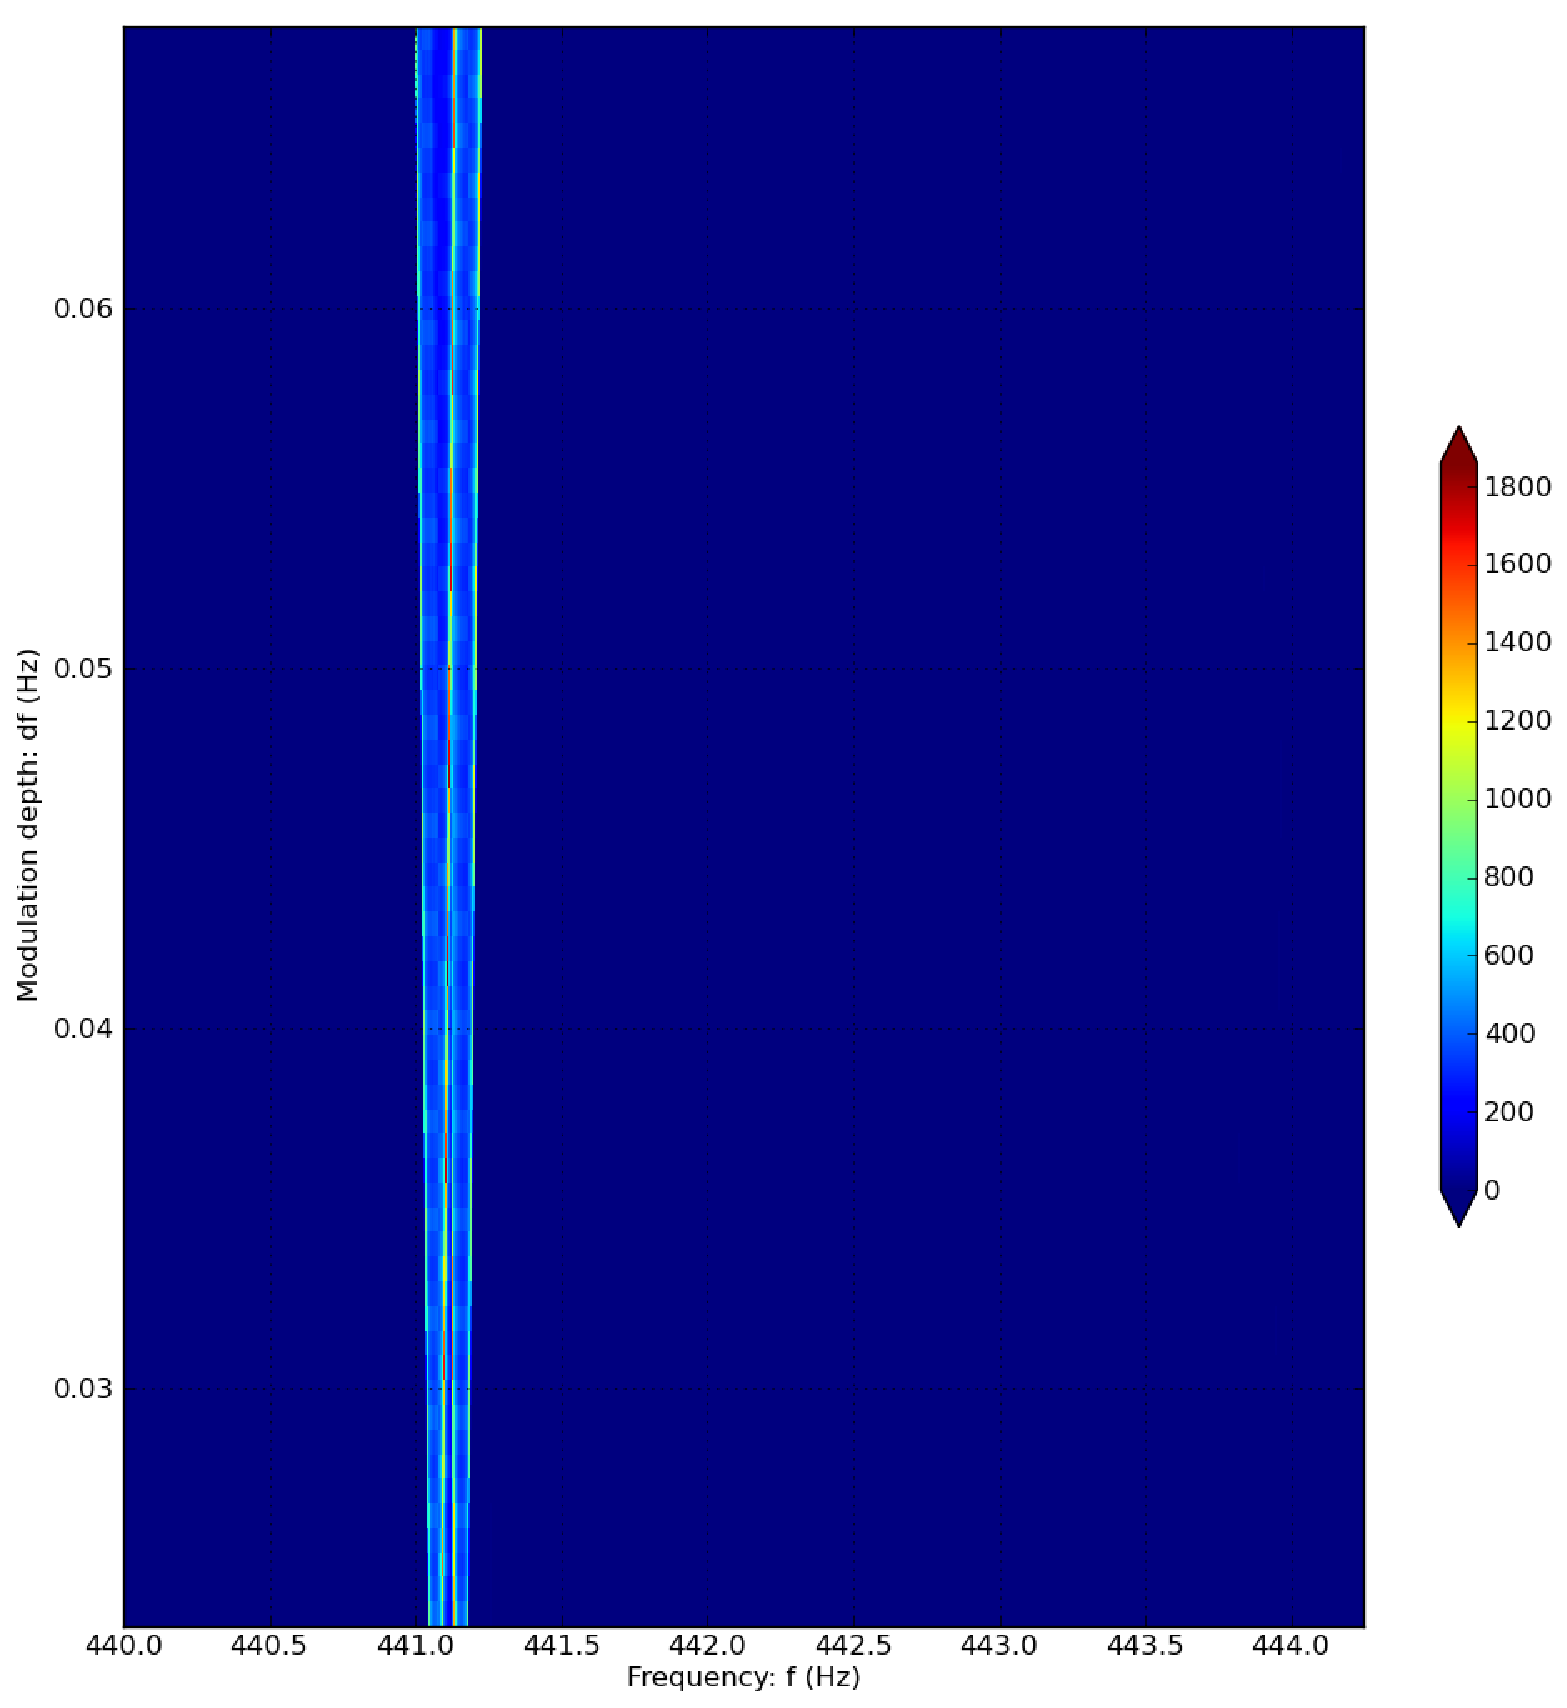
\includegraphics[width=0.65\paperwidth,height=0.5\paperheight]{plots/bandH1-bold.eps}
\caption{
Scorpius X-1 Mock Data Challenge (MDC) pulsar 40 \{H1\}: 5 Hz band. 
The $-\log_{10}p$-value (single-template, applying Davies' Method to the $R$ statistic) is shown in this heatmap, peak in red. 
All templates are plotted on the (frequency, modulation depth) plane.
This is a relatively broadband view.
}
\label{scox1-wide-heatmap-040}
\end{center}
\end{figure}


Figure~\ref{scox1-wide-heatmap-040} shows the result of a 5 Hz-wide analysis on an easily detectable pulsar.

\begin{figure}
\begin{center}
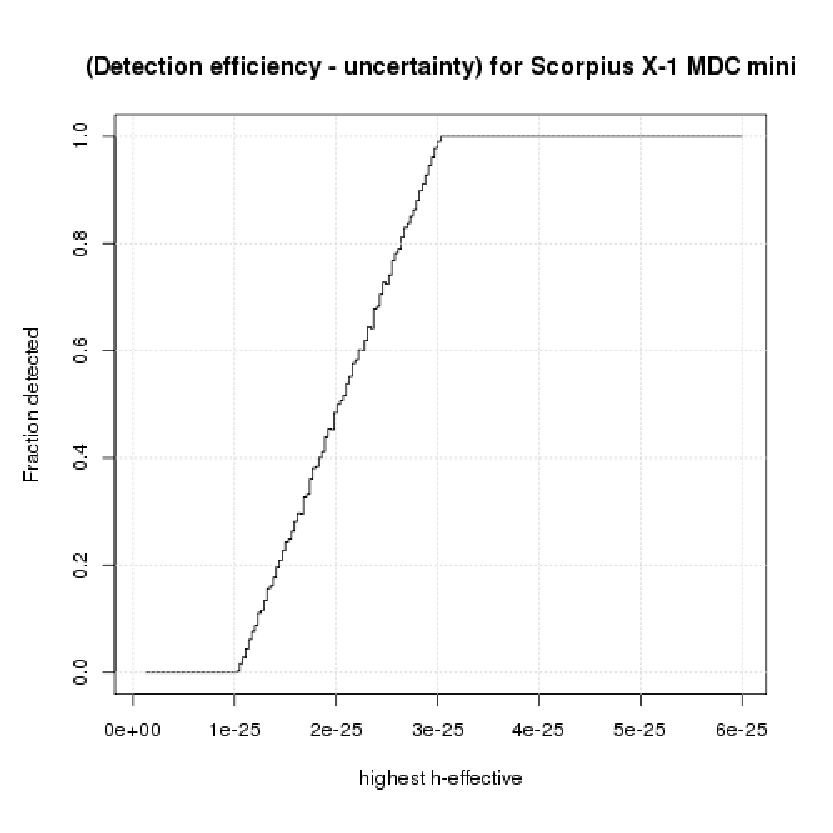
\includegraphics[trim=0 10 10 5, clip, width=0.70\paperwidth,height=0.48\paperheight]{plots/PlotHeffDistH0DetectionEfficiency200breaks.eps}
\caption{ Simulated detection efficiency curve. Because the $\cos \iota$ ambiguity simulation require a priori model of detection efficiency, we describe it simply. Here, no detections are claimed below $1\times 10^{-25}$, all are detected above $3\times 10^{-25}$, and the probability of detection rises uniformly on the intervening interval.
\label{fig:plotheffdisth0detectionefficiency200breaks}}
\end{center}
\end{figure}

\subsection{Sensitivity depth}
\label{sensitivity-depth-appendix}

Sensitivity depth answers whether an analyses has the power to see a certain strain in detector data.
GW observatory data has an amplitude spectral density, $S_H^{1/2}(f)$.
The minimum $S_H^{1/2}(f)$ was about $2\times 10^{-23}\mathrm{~Hz}^{-1/2}$ in initial LIGO or $4\times 10^{-24}$ $\mathrm{~Hz}^{-1/2}$ in Advanced LIGO~\cite{HarryALIGO2010}, which should be achieved in the 100-300 Hz band.
%Coherent searches are the most sensitive in terms of \textit{sensitivity depth}, or power to resolve signals for a given noise spectral sensitivity.
Define the depth as $D$,

\begin{equation}
D(f) \equiv \frac{S_H^{1/2}(f)}{h_0(f)},
\end{equation}

\noindent for an $h_0(f)$ at a specified confidence level and frequency.
In LIGO S4 data, the Hough, StackSlide, and PowerFlux methods achieved 95\%-confidence upper limits on $h_0$ of approximately $4.3\times 10^{-24}$,
% in noise of $2.5 \times 10^{-19} \mathrm{~m~Hz}^{-1/2}$, 
or $6.25\times 10^{-23} \mathrm{~Hz}^{-1/2}$,
a sensitivity depth of about 15$\mathrm{~Hz}^{-1/2}$,
and improvements have been made since this comparison~\cite{LSCPulsarS4}.
Complications for coherent searches, such as spin-wandering, unknown orbital parameters, and sky location, motivated the development of TwoSpect.
In the all-sky search of S6 data~\cite{GoetzTwoSpectResults2014}, the most constraining 95\%-confidence upper limit of $2.3\times10^{-24}$ (assuming circularly-polarized GW) was achieved in a detector noise floor around $2\times 10^{-23} \mathrm{~Hz}^{-1/2}$~\cite{Fricke2009}, implying a sensitivity depth around 10$\mathrm{~Hz}^{-1/2}$ for circular polarization.
Searching for unknown sources across the sky is justified: GWs theoretically less directional than beamed X-ray flux, so sources with GW luminosity equal or greater than Sco X-1 might be as-yet unknown in electromagnetic counterparts.
Yet the all-sky search~\cite{GoetzTwoSpectMethods2011} parameter space is too large to search at full sensitivity.
Sco X-1, conversely, allows a directed search at its sky location, projected semi-major axis and orbital period.
Fully template-testing the reduced parameter space is intended to yield enhanced sensitivity depth.


    \subsection{Signal model}
    \label{signal-model-appendix}

%\textbf{Signal model}\\

Gravitational waves from a neutron star in a binary system are described by strain as a function of time $h_0(t) = h_0 e^{i \Phi(t)}$. 
Measured strain $h(t)$ depends on the detector response to $h_0(t)$.
Amplitude $h_0$ depends on the astrophysical parameters of the neutron star~\cite{Jaranowski1998}.
The phase model $\Phi$ can be described using detector time $t$ and Solar System Barycenter (SSB) time $t_\mathrm{SSB}$.
Travel from the source to SSB introduces an overall phase shift; uncertainty in the distance and proper motion is systematic and the same for gravitational and electromagnetic observations.
Detector time is recorded in GPS time, running parallel with Terrestrial Time (TT), and SSB time runs parallel with Barycentric Dynamical Time (TDB). 
SSB time corrects $t$ by $\delta t_R$ for relativistic effects.
Another overall phase shift is caused by  Roemer delay $\Delta t_R$, the dot product of $\hat{n}/c$ from the SSB to the sky location of interest with $\vec{r}$ from the SSB to the detector~\cite{Jaranowski1998,GoetzTwoSpectMethods2011,TwoSpectCoherentGoetz2015}.
Barycentering detector-frame data is equivalent to resampling in $\tau(t) = t_\mathrm{SSB}(t) + \Delta t_R(t)$, 

% OLD STUFF BELOW
%The phase model $\Phi$ can be described using detector time $t$ and Solar System Barycenter (SSB) time $t_\mathrm{SSB}$.
%The Lorentz dilation is $\gamma= \sqrt{1+(v/c)^2}\approx 5\times 10^{-9}$ for the Earth's motion.
%Gravitational time dilation is $\sqrt{1-2GM/(rc^2)}$ and of comparable magnitude with opposite sign. 

\begin{equation}
\tau(t) 
% &= \gamma + \Delta t_R, \\ 
 = t + \frac{\vec{r}(t) \cdot \hat{n}}{c} + \delta t_R.
\label{barycentering_time_domain}
\end{equation}

Binary motion can be described as modulating GW emission frequency $f=f_0$ by the orbital motion of the companion object~\cite{GoetzTwoSpectResults2014}.
The frequency $f$ is usually presumed equal to $2\nu_s$ for a neutron star spin frequency of $\nu_s$, as it would be for quadrupolar radiation due to ellipticity on the star.
Orbital modulation occurs at a frequency $\Omega = 2\pi/P$ with a frequency modulation depth $\Delta f_\mathrm{obs}$,

\begin{equation}
\Delta f_\mathrm{obs} = \frac{2 \pi f_0 \cdot (a \sin i)}{cP}.
\label{TwoSpect_mod_depth}
\end{equation}

\noindent The binary system's projected semi-major axis is $a \sin i$, inclined by the angle $i$ of the orbital axis measured with respect to the observer's line-of-sight; $P$ is the orbital period of the system.
It is useful to express $a \sin i$ in light-seconds.
Orbital phase is specified by $T_\mathrm{asc}$, the SSB time of ascension, when the companion object crosses the ascending node; the phase can nevertheless be stated as a function of detector time $t$.
Future work may consider eccentricity $e$, but it was considered small enough to not be simulated in our comparison~\cite{ScoX1MDC2015PRD}.
Reference time is established by $\Phi(T_\mathrm{ref}) = \Phi_0$.
An unknown spin-wandering term, $\delta \Phi_\mathrm{spin-wander}$, is hypothesized.

Phase $\Phi$ can thus be expressed in $t$, using $\tau_B$ to resample the binary motion: 

\begin{equation}
\tau_B(t) \equiv \tau(t) + [a \sin(i)/c] \sin (\Omega [t - T_\mathrm{asc}]),
\label{resampled_time}
\end{equation}
\begin{eqnarray}
\Phi(t) 
    &= \Phi_0 &+ \delta \Phi_\mathrm{spin-wander} + 2\pi f_0 \cdot \left(\tau_B(t) - T_\mathrm{ref}\right), \label{compact_phase_model} \\
    &= \Phi_0 &+ \delta \Phi_\mathrm{spin-wander} \nonumber\\
    & &+ 2\pi \left[f_0 \cdot \left(\tau(t)-T_\mathrm{ref}\right) + \frac{\Delta f_\mathrm{obs}}{\Omega} \sin (\Omega [t - T_\mathrm{asc}]) \right], \\
    &= \Phi_0 &+ \delta \Phi_\mathrm{spin-wander} \nonumber\\
    & &+2\pi \left[f_0 \cdot \left(t + \frac{\vec{r}(t)\cdot \hat{n}}{c}+\delta t_R-T_\mathrm{ref}\right)\right] \nonumber\\
    & &+2\pi \left[ \frac{\Delta f_\mathrm{obs}}{\Omega} \sin (\Omega [t - T_\mathrm{asc}]) \right].
\label{phase_model}
\end{eqnarray}


Strain as a function of time, $h(t)$, is expected to be present in two polarizations, \textit{plus}, $h_+$, and \textit{cross}, $h_\times$.
Our analyses uses $h(t)$ from a single detector that responds to both polarizations, depending on right ascension $\alpha$, declination $\delta$, time $t$ and polarization angle $\psi$, with functions $F_+$ and $F_\times$.
The $F_+$ and $F_\times$ also depend on detector geographical location and orientation.
The proportion of the signal in each polarization is determined by the polarization angle $\iota$ of the neutron star rotation axis with respect to the line of sight of the observer.
Antenna-pattern response is calculated by projecting the polarization tensor, for $\psi$ and sky location, onto the detector~\cite{YunesSiemens2013}.
Antenna response is represented by the covector $F_j$ with components $(F_+, F_\times)$:

\begin{eqnarray}
F_j(t,\alpha,\delta,\psi) 
%\equiv 
%\left( \begin{array}{rr} F_+(t, \alpha, \delta, \psi)  & F_\times(t, \alpha, \delta, \psi) \end{array} \right) \nonumber \\
=
\left( \begin{array}{rr} \cos 2 \psi & \sin 2 \psi \end{array} \right) \left( \begin{array}{cc} a(t, \alpha, \delta) & b(t, \alpha, \delta) \\ b(t, \alpha, \delta) & -a(t, \alpha, \delta) \end{array}\right)   ,
\end{eqnarray}

\noindent where detector specific responses $a$ and $b$ depend on ($\alpha,\delta$) and location~\cite{Jaranowski1998}. Incident GW polarization is $\iota^j_k J^k$, acting on the Jones vector $J^k$:
%
%\begin{equation} 
%\textbf{h}_j = h_0 (\iota_{jk} \Phi_k),
%\end{equation}
%
%\noindent where
%
\begin{eqnarray}
\iota^j_k =
\left(
\begin{array}{cc}
\frac{1+\cos^2 \iota}{2} & 0 \\
0 & \cos \iota \\
\end{array}
\right),\\
J^k = \left(
\begin{array}{c}
1\\
-i\\
\end{array}
\right).
\end{eqnarray}

\noindent The phases of the two polarizations are expressed by the vector $\Phi^k(t)$:

\begin{eqnarray}
\Phi^k(t) =
\Re\left[J^k e^{\mathrm{i} \Phi(t)} \right]
=
\left(
\begin{array}{c}
\cos \Phi(t)\\
\sin \Phi(t)\\
\end{array}
\right).
\end{eqnarray}

\noindent It is convenient to factorize $\mathcal{A}_k \equiv h_0 \cdot (F_j \iota^j_k)$~\cite{TwoSpectCoherentGoetz2015} and to introduce $A \equiv (\mathcal{A}_+ - \mathrm{i} \mathcal{A}_\times )/2$. 
Note $A = (1/2)h_0 \cdot (F_j \iota^j_k J^k)$. 
Complex conjugate $*$ yields a compact waveform expression.
Gathering terms, the expected GW strain model is $h(t)$:

\begin{eqnarray}
h(t)
 &= \mathcal{A}_k \Phi^k, \\
 &= \Re\left[h_0 F_j \iota^j_k J^k e^{\mathrm{i}\Phi(t)}\right], \\
  &= A e^{\mathrm{i}\Phi(t)} + A^* e^{-\mathrm{i}\Phi(t)}, \label{Evan_expression_ht}\\
%h(t) 
&= h_0 F_+ \frac{1+\cos^2 \iota}{2}\cos \Phi(t) +
  h_0 F_\times \cos \iota \sin \Phi(t).
\label{amplitude_model}
\end{eqnarray}

\noindent Circular polarization, when $\cos \iota =1$, maximizes $h(t)$, though $\iota$ is often unknown.

%Although one can interpret $F_j$, $\iota^j_k$, and $\Phi^k$ in several ways, the core 
Searches for $h(t)$ can model $\Phi(t)$, where $\iota$ and $\psi$ are often nuisance parameters and the strain amplitude $h_0$ is later inferred.
The response $F_j$ decomposes to a unit-vector right-multiplied by the (transverse-traceless) detector response matrix. 
This detector matrix can be interpreted as a metric for the inner product $h(t)$ of the polarization tensor and the Jones vector.
We compose $F_j$ with the (diagonal) dilation-rotation $\iota^j_k$ to produce $A$.
Equation~\ref{Evan_expression_ht} illustrates that $A$ is half the modulus, and $\Phi$ the argument, of $h(t)$; this formalism generalizes to include multiple detectors~\cite{TwoSpectCoherentGoetz2015}. 
The measured output $x(t)$ of a detector corresponds to the signal $h(t)$ plus noise $n(t)$,

\begin{equation}
x(t) = h(t) + n(t).
\end{equation}

        \subsection{TwoSpect statistics}
        \label{all-sky}

The TwoSpect program calculates a test statistic $R$ and single-template $p$-value for a putative template waveform of a neutron star emitting continuous GWs in a binary system.
The construction of this $R$-statistic can be described in several steps.
Science/observing runs are first parcelled into overlapping short Fourier transforms (SFTs), performed in the detector frame.
The SFTs have typical coherence time $T_\mathrm{SFT}$, also referred to as $T_\mathrm{coh}$ in past work, ranging from 60 s to 1800 s, depending on the hypothesized time-derivative of neutron star frequency~\cite{GoetzTwoSpectMethods2011}.
The total number of SFTs with 50\%-overlap for an observing time $T_\mathrm{obs}$ is $N$,

\begin{equation}
N = \mathrm{floor}\left(\frac{2 T_\mathrm{obs}}{T_\mathrm{SFT}}\right) - 1.
\end{equation}

\noindent SFT number in the observing run are indexed by $n \in [0,\ldots,N-1]$; SFT frequency bin is indexed by $k \in [0,\ldots,K -1]$, where $K = T_\mathrm{SFT} f_N$ for a Nyquist frequency $f_N$ and only positive frequencies $k = T_\mathrm{SFT} f$ are used. 
Thus the transformation from time series to SFTs is a map from $x(t)$ (containing $h(t)$) to $\tilde{x}^n_k$.

Each SFT frequency bin $\tilde{x}^n_k$ is Doppler shifted to a frequency bin in the SSB frame corresponding to the sky location, frequency, and time $t$ of the midpoint of the SFT $n$ under investigation: $k(f(\alpha,\delta,t)) \rightarrow k(f_\mathrm{SSB}(\tau))$.
This barycentering procedure corresponds to the time-domain Equation~\ref{barycentering_time_domain}.
Figure~\ref{tfplane-figure}
shows a simulated signal in the resulting time-frequency plane.
Henceforth, barycentering is implicit in the $k$ index.
Define the power $P^n_k = 2|\tilde{x}^n_k|^2/T_\mathrm{SFT}$.
Let $\left<P_k\right>^n$ be the expected (estimated from a running mean over nearby $n$) noise-only power in a frequency bin $k$ for SFT $n$.
Also let $F^2_n \equiv F_{+,n}^2 + F_{\times,n}^2$ for the antenna pattern at the chosen sky location and SFT $n$ -- taking this equal-weighted sum implies an assumption of circular polarization. 
Then the estimated power in a given bin $\tilde{P}^n_k$ is normalized such that random, white, Gaussian noise will have an expectation value of 1~\cite{GoetzTwoSpectMethods2011}:

\begin{equation}
\tilde{P}^n_k = \frac{F_n^2 (P_k^n - \left<P_k\right>^n)}{(\left<P_k\right>^n)^2}\left[\sum\limits_{n'}^N \frac{F_{n'}^4}{(\left<P_k\right>^{n'})^2} \right]^{-1}.
\label{equation_with_antenna_pattern}
\end{equation}

Then each row of barycentered frequency bins $k$ is treated as a time series in $n$.
Power for bin $k$ in that time series is Fourier transformed by $\mathcal{F}_{f'}$ into $Z_k(f')$ (Figure~\ref{ffplane-figure}), where $f'$ is the second Fourier transform frequency.
During the transform, the background noise power $\lambda(f')$ is estimated from the noise in the SFTs, assuming the noise is Gaussian.
This second Fourier power $Z_k(f')$ follows a $\chi^2$ distribution with 2 degrees of freedom and mean 1.0, is proportional to $h^4$, and is constructed by 

\begin{equation}
Z_k(f') = \frac{\left| \mathcal{F}_{f'} [\tilde{P}^n_k]  \right|^2}{\left< \lambda(f') \right>}.
\label{second_Fourier_power}
\end{equation}

At this point it is helpful to explicitly define how the background is constructed.
An average noise ratio per frequency bin, $\rho_k$, is defined by

\begin{equation}
\rho_k = \frac{\sum_{n=0}^{N-1} \left(\left<P_k\right>^n\right)^{-1}}{\sum_{n=0}^{N-1} \left(\left<P_k\right>^n\right)^{-2}} \left(\frac{1}{K} \sum_{k=0}^{K-1} \sum_{n=0}^{N-1} \left(\left<P_k\right>^n\right)^{-1} \right).
\end{equation}

\noindent Designate the median, over $k$, of $\left<P_k\right>^n$ as $\mu_n$.
A random variable $Y$, drawn from an exponential distribution according to $\mu_n$ and used to construct a simulated time-frequency power $X_n$:

\begin{equation}
X_n(Y_q) = \left(\frac{(Y_q)}{\mu_n} - 1 \right) \times \frac{F_n^2}{\mu_n} \left[ \sum\limits_{n'=0}^{N-1} \frac{F_{n'}^4}{(\mu_{n'})^2} \right].
\end{equation}

\noindent We then compute the average noise in each of $F' = (\mathrm{floor}(N/2) +1)$ second-frequency bins $f'$.
A Monte Carlo simulation with $T$ trials, typically 4000, generates the random variable $Y$.
The $Y$ are indexed by trial $q$.  
The simulation computes the un-normalized average noise $\lambda(f')$, with mean $\left< \lambda(f') \right>$:

\begin{eqnarray}
\lambda(f') = \frac{1}{T} \sum_{q=0}^{T-1}|\mathcal{F}_{f'}\left(X_n (Y_q)\right)|^2.
\end{eqnarray}

\noindent The background power of a pixel, used later in constructing test-statistics, is $\lambda_k(f')$:

\begin{equation}
\lambda_k(f') = \rho_k \frac{\lambda(f')}{\left< \lambda(f') \right>}.
\end{equation}

Signal templates encode the expected $h(t)$ into pixel weights $w$. 
Weights are applied to pixels on the frequency-prime $f'$ vs frequency $f$ plane to give the test statistic $R$; the directed search uses templates defined in the $f$ vs $t$ plane by $x$, then Fourier-transformed into $w$. 
A template has a requested length, $M$, and pixels are indexed by $i \in [0,M-1]$ pixels such that $w_0$ is largest and $w_i \geq w_{i+1}$.
Weights are normalized such that the sum of $w_i$ equals one.
The exact templates depend on SFT number $n$, frequency bin $k$ corresponding to $f_0$, frequency bin $z$ of interest, and SFT coherence time midpoint $T_m$.

Calculating the templates involves Taylor expansion for the coherence time of an SFT, then Fourier transforming a sampled time series.
A dot denotes $d/dt$.
Let $t_B \equiv t + [a \sin (i)/c]\sin(\Omega[t-T_\mathrm{asc}])$, so $\dot{t}_B = 1 + [\Delta f_\mathrm{obs}/f] \cos(\Omega [t_m-T_\mathrm{asc}])$.
Then $\dot{\tau}_B = \dot{t}_B + \frac{d}{dt}(\Delta t_R +\delta t_R)$.
Expand $\Phi(t_m)$ from Equation~\ref{compact_phase_model} about $t_m$:

\begin{equation}
\dot{\tau}_B = 1 + \frac{\vec{v}(t_m) \cdot \hat{n}}{c} + \frac{d}{dt}\delta t_R+ \frac{\Delta f_\mathrm{obs}}{f_0} \cos \left(\Omega [t - T_\mathrm{asc}]\right),
\label{tau-time-derivative}
\end{equation}
\begin{eqnarray}
\Phi(t_m) &\approx \Phi_0 &+ \delta \Phi_\mathrm{spin-wander} \nonumber \\
  & &+ 2 \pi f_0 \left(t_m + \frac{\vec{r}(t_m)\cdot \hat{n}}{c} +\delta t_R- T_\mathrm{ref} + \dot{\tau}_B \cdot [t-t_m] \right). 
\end{eqnarray}

\noindent Indexing $L = 2f_\mathrm{Nyquist}T_\mathrm{SFT}$ time samples by $l\in [0,\ldots,L-1]$, we can gather constant terms into $\hat{\Phi}$.
Then take the Fourier transform $\tilde{h}_k \equiv \mathcal{F}_k(h(t))$ of positive frequencies in the signal model, Equation~\ref{Evan_expression_ht}, allowing windowing weights $u_l$ with $C\equiv\left(\sum_{l=0}^{L-1} u_l^2 / L \right)^{1/2}$:

\begin{eqnarray} 
\hat{\Phi} &\equiv \Phi_0 &+ \delta\Phi_\mathrm{spin-wander} \nonumber\\
  & &+ 2\pi f_0 \left(t_m + \frac{\vec{r}(t_m)\cdot\hat{n}}{c} +\delta t_R- T_\mathrm{ref} - \dot{\tau}_B t_m\right),
\end{eqnarray}
\begin{eqnarray}
\tilde{h}_k 
  &= \frac{T_\mathrm{SFT}}{CL} \sum\limits^{L-1}_{l=0} u_l A e^{\mathrm{i} \left(\hat{\Phi} + 2\pi f_0 \dot{\tau}_B [l T_\mathrm{SFT}/L]\right)} e^{- 2\pi \mathrm{i} [lk /L]},\\ 
%  &= \frac{T_\mathrm{SFT}}{CL} \sum\limits^{L-1}_{l=0} u_l A e^{\mathrm{i} \hat{\Phi}} e^{2 \pi \mathrm{i} \left(f_0 \dot{\tau}_B T_\mathrm{SFT} - k\right)l/L},\\
  &= A e^{\mathrm{i} \hat{\Phi}} \frac{T_\mathrm{SFT}}{CL} \sum\limits^{L-1}_{l=0} u_l \left[e^{2\pi \mathrm{i} \left(f_0 \dot{\tau}_B t_\mathrm{SFT} - k\right)/L} \right]^l.
\label{Fourier_transform_of_signal}
\end{eqnarray}

\noindent Equation~\ref{Fourier_transform_of_signal} contains a geometric series that converges in the large $L$ limit to a Dirichlet kernel~\cite{TwoSpectCoherentGoetz2015}.
Defining $\delta_k \equiv \left(f_0 \dot{\tau}_B T_\mathrm{SFT} - k\right)$, the kernel $D_h$ for the typical Hann window, C = $\sqrt{3/8}$, yields the Fourier transform of the signal model precisely:

\begin{equation}
D_h (\delta_k) = \frac{\mathrm{i} e^{2\pi \mathrm{i} \delta_k} - \mathrm{i}}{4\pi \delta_k \left[(\delta_k)^2 - 1 \right]},
\end{equation} 
\begin{equation}
\tilde{h}_k = A e^{\mathrm{i} \hat{\Phi}} \frac{T_\mathrm{SFT}}{C} D_h \left( \delta_k \right).
\end{equation}

\noindent taking the power $|\tilde{h}_k|^2 = \tilde{h}_k^*\tilde{h}_k$, and defining a coefficient $r_{1/2}= h_0^2 \cdot (\mathcal{A}_+^2 + \mathcal{A}_\times^2)\cdot T_\mathrm{SFT}^2$ along with $\mathrm{sinc}(x) \equiv \sin (\pi x)/ (\pi x)$,

\begin{eqnarray}
|\tilde{h}_k|^2 &= \frac{h_0^2}{4} \cdot (\mathcal{A}_+^2 + \mathcal{A}_\times^2)\cdot\frac{T_\mathrm{SFT}^2}{3/8} \left|\frac{2 - 2 \cos(2\pi \delta_k)}{16 \pi^2 \delta_k^2 [\delta_k^2 -1]^2} \right|,\nonumber \\
 &= \frac{r_{1/2}}{4} \frac{2}{3} \frac{\mathrm{sinc}^2\left(\delta_k\right)}{[\left(\delta_k \right)^2-1]^2}.
\label{modern_tfplane_template_power}
\end{eqnarray} 

Equation~\ref{modern_tfplane_template_power}, multiplied by $4$ to normalize for having taken positive frequencies only, corresponds to previous calculations for Hann-windowed power $|x_z(n)|^2$ in a pixel in the time-frequency plane~\cite{GoetzTwoSpectMethods2011}:
%Code is available online~\cite{LALAPPSrepo}.

\begin{equation}
|x_z (n)|^2 = \frac{2}{3} \frac{\mathrm{sinc}^2\left[k + \Delta f_\mathrm{obs} T_\mathrm{SFT} \sin (2\pi n T_m/P) - z \right]}{\left[ (k + \Delta f_\mathrm{obs} T_\mathrm{SFT} \sin (2\pi n T_m / P) - z)^2 - 1 \right]^2},
\label{methods_paper_template_power}
\end{equation}

\noindent where $z$ is now independent instead of $k$, which denotes the bin of the central frequency. 
Substituting $\sin(2\pi nT_m/P) \leftrightarrow \cos(\Omega [t-T_\mathrm{asc}])$ is permitted, because taking the second Fourier power with Equation~\ref{second_Fourier_power} removes the orbital phase information, $T_\mathrm{asc}$.
Comparing Equation~\ref{modern_tfplane_template_power} to previous calculations, Equation~\ref{equation_with_antenna_pattern} normalizes $r_{1/2}$, while $f_0 \dot{\tau}_B T_\mathrm{SFT}= k_0 + \Delta f_\mathrm{obs} T_\mathrm{SFT} \cos(\Omega [t-T_\mathrm{asc}])$, when $k_0\equiv f_0 \cdot (1+\vec{v}(t_m)\cdot\hat{n}/c + (d/dt)\delta t_R)\cdot T_\mathrm{SFT}$.
The $k_0$ is the barycentered discrete frequency bin.
These substitutions give Equation~\ref{methods_paper_template_power}, which corresponds analytically to the simulated power of pixels in Figure~\ref{tfplane-figure}.
Fourier transform \textit{two} in TwoSpect follows, integrating over SFT number $t$ for $N$ SFTs with a Hann window $u_n$:
this is the expression computed in code,

\begin{equation}
\mathcal{F}_{f'}(\left|x_z(n) \right|^2) = \frac{1}{CN} \sum\limits_{n=0}^N \left[u_n e^{-2\pi \mathrm{i} n f'/N} \left|x_z(n)\right|^2\right].
\label{fourier_transform_of_tfplane_power}
\end{equation}

Values of $\mathcal{F}_{f'}(\left|x_z(n) \right|^2)$ are numerically integrated.
The values are squared, $w_{z}(f') \equiv \left| \mathcal{F}_{f'}(\left|x_z(n) \right|^2) \right|^2$, then sorted for magnitude (over $z$ and $f'$) into the $M$ largest values of $z(i)$, $f'(i)$, indexed by $i$.
The exact template weights are defined $w_i \equiv w_{z(i)}\left(f'(i)\right) / \Sigma_i w_{z(i)} \left(f'(i) \right)$, so that $(w_i \geq w_{i+1}) \forall i\in [0,\ldots, M-1]$ and $\Sigma_i w_i = 1$.
The corresponding second-Fourier power terms are chosen, $Z_i \equiv Z_{z(i)}\left(f'(i)\right) = \left|\mathcal{F}_{f'(i)}[|x_{z(i)}(n)|^2] \right|^2/\left<\lambda(f') \right>$.

% Template weights $w_i$ can be approximatedly quickly by using a Gaussian pulse train.
% DETAIL this procedure? NOT NEEDED as Evan confirms we use exact templates

\begin{figure}
\begin{center}
%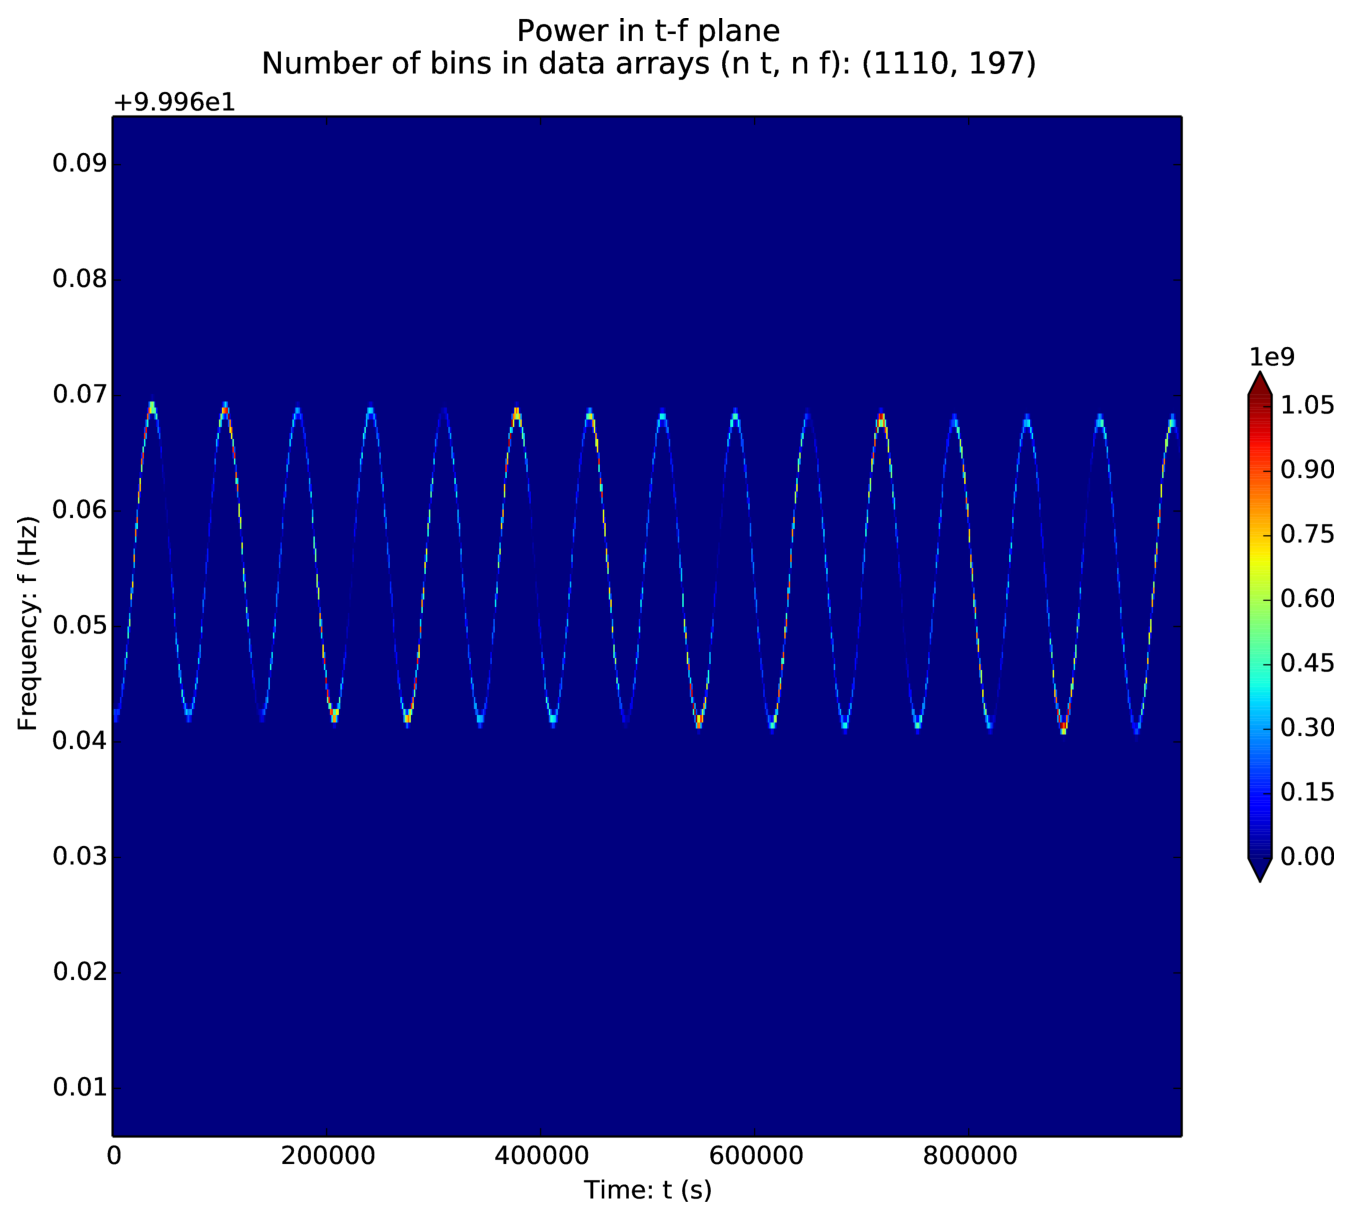
\includegraphics[trim=20 15 80 40, clip, keepaspectratio,height=0.35\paperheight]{plots/tfplane-4e21-on-4e24.eps}
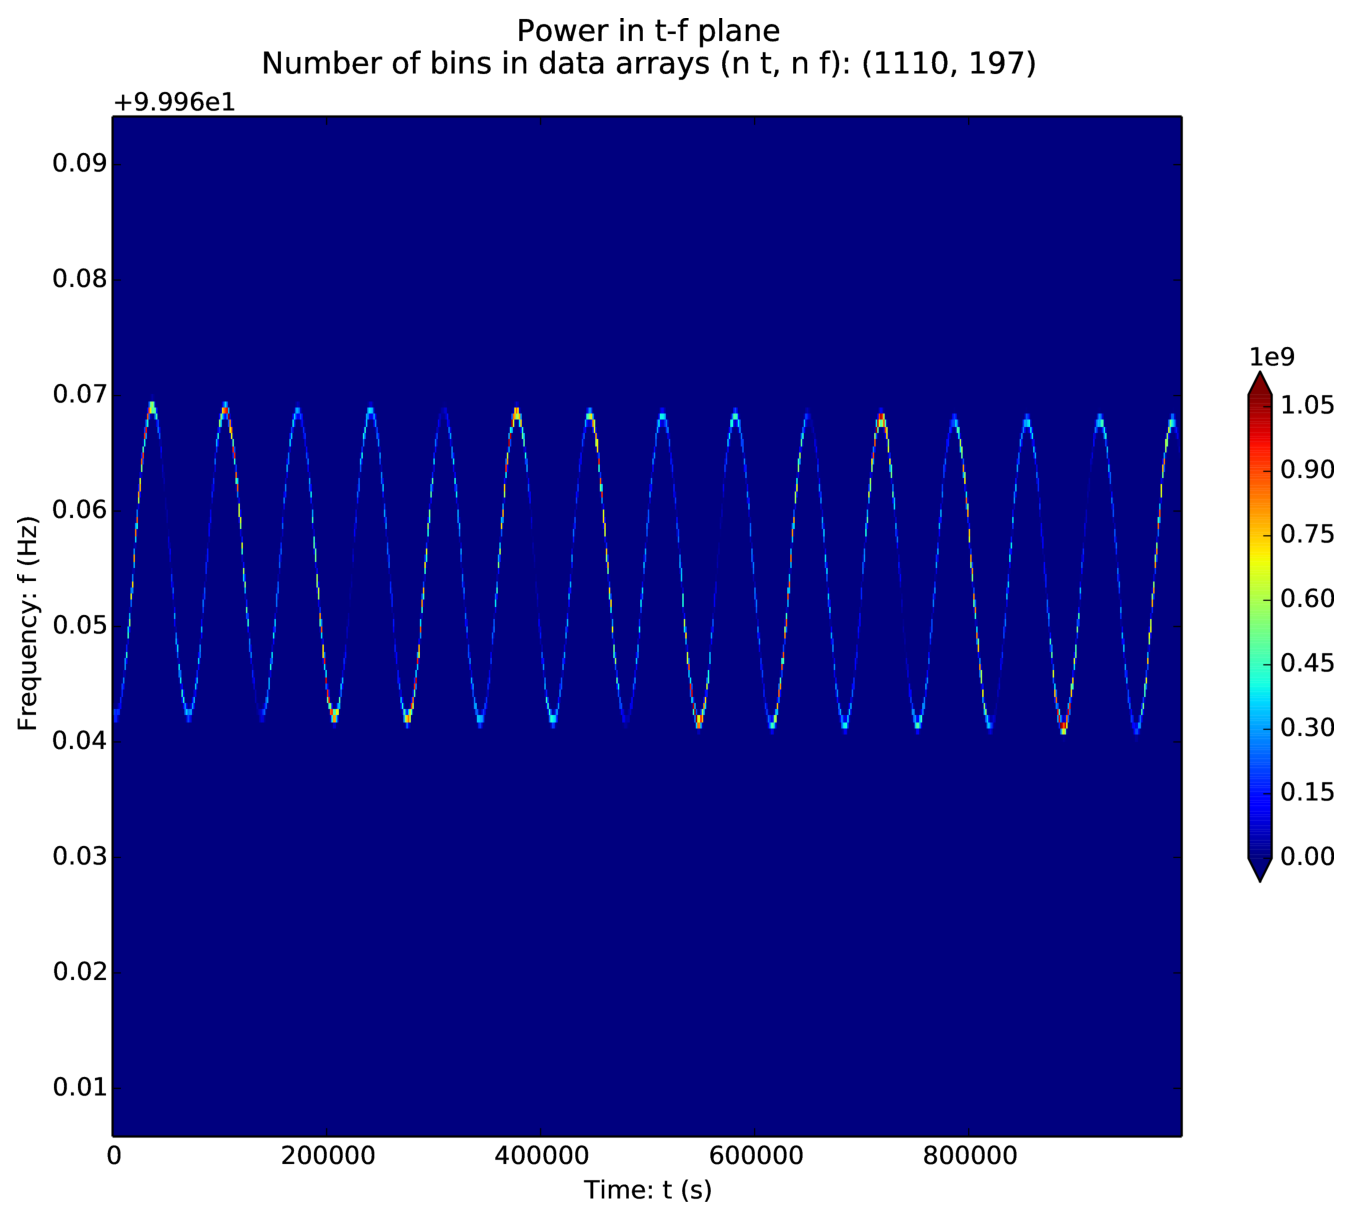
\includegraphics[keepaspectratio,height=0.35\paperheight]{plots/tfplane-4e21-on-4e24.eps}
\caption{By Doppler-shifting the frequencies into the solar system barycenter, TwoSpect makes this $f$ vs $t$ plane (pixel color indicates power). A simulated signal at 100.015 Hz with $P = 68023.8259$ s and $\mathrm{a} \sin i = 1.44$ modeling Sco X-1 is injected with $h_0 = 4\times 10^{-21}$ into $10^6$ s of Gaussian noise at $S^{1/2}_{h} = 4 \times 10^{-24}$ Hz$^{-1/2}$ (projected minimum Advanced LIGO noise).}
\label{tfplane-figure}
\end{center}
\end{figure}

\begin{figure}
\begin{center}
%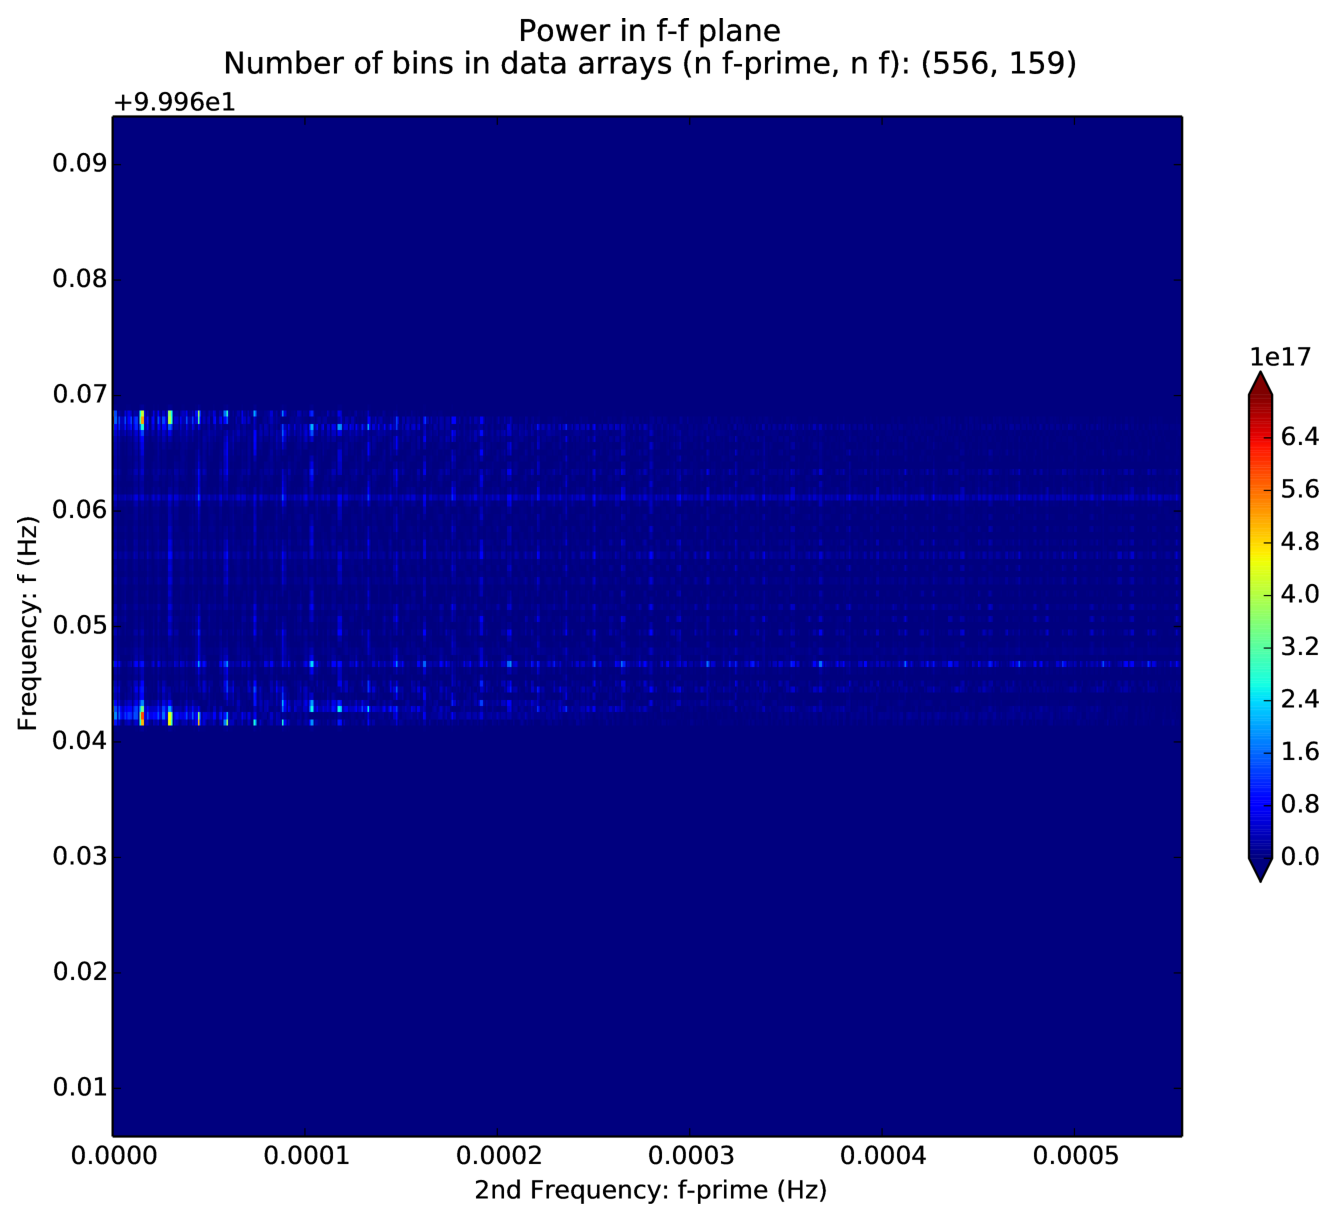
\includegraphics[trim=20 15 80 40, clip, keepaspectratio,height=0.35\paperheight]{plots/ffplane-4e21-on-4e24.eps}
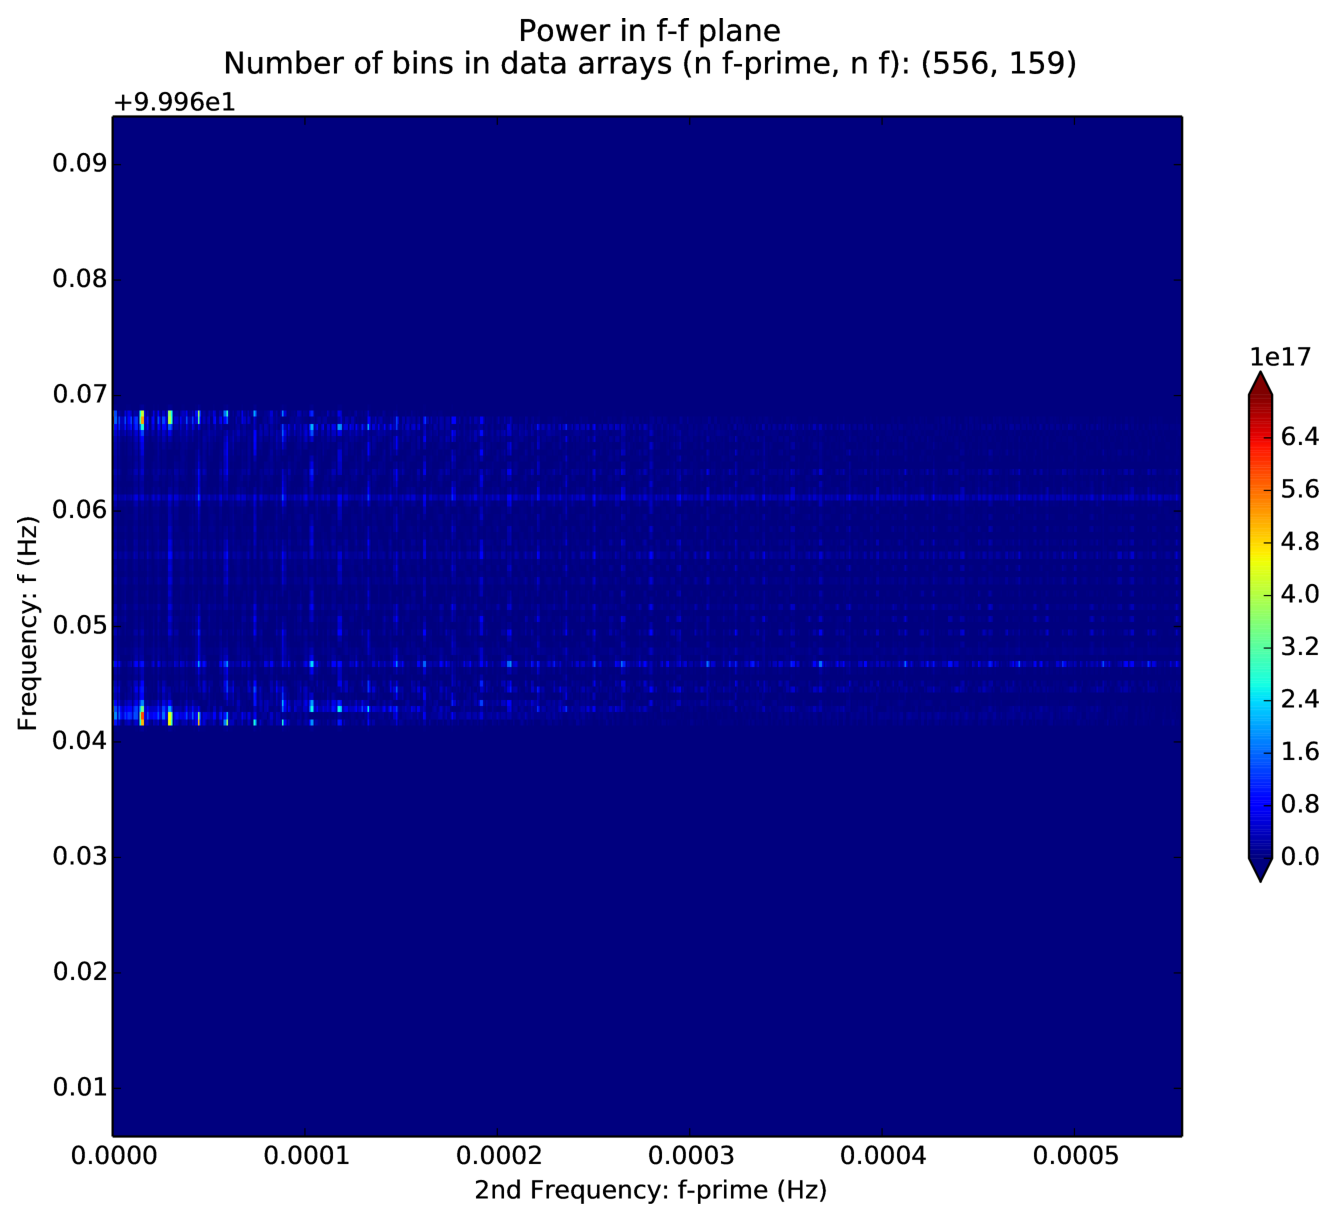
\includegraphics[keepaspectratio,height=0.35\paperheight]{plots/ffplane-4e21-on-4e24.eps}
\caption{Fourier-transforming along the time bins of each frequency row yields the $f$ vs $f'$ plane (pixel color indicates power). Templates are matched against pixels to compute the $R$ statistic. NOTE: the $x$-axis label is in fact \textit{bin number} and each value is the 2nd Fourier frequency in Hz times 1800 s.}
\label{ffplane-figure}
\end{center}
\end{figure}

%            \subsection{Inferring neutron stars with companions}
%            \label{inference}
 
Templates only vary for GW emission frequency $f$ and projected semi-major axis $a \sin i$, if orbital period $P$ and sky location are known.
%Projected semi-major axis manifests as a GW frequency modulation depth $\Delta f$~\cite{GoetzTwoSpectMethods2011},
%\begin{equation}
%\Delta f = \frac{2 \pi f (a \sin i)}{c P},
%\label{TwoSpect_mod_depth}
%\end{equation}
TwoSpect calculates an $R$ detection statistic~\cite{GoetzTwoSpectMethods2011} by taking the normed inner product of template weights $w_i$ with background $\lambda_i$-subtracted second-Fourier power $Z_i$ (Equation~\ref{TwoSpect_R_statistic}).

\noindent Define the inner product $<\vec{u}, \vec{v}>$, with norm squared $||\vec{u}||^2 \equiv <\vec{u}, \vec{u}>$ and projection $\mathit{proj}_{\vec{u}} \vec{v} \equiv ||\vec{u}||^{-2} <\vec{v}, \vec{u}> \vec{u}$:

\begin{eqnarray}
<\vec{u}, \vec{v}> \equiv \sum_{i=0}^{M-1} u_i v_i,\\
R = ||\vec{w}||^{-2} \cdot \left<\vec{w}, (\vec{Z} - \vec{\lambda})\right>,\\
\mathit{proj}_{\vec{w}} \left(\vec{Z} - \vec{\lambda} \right) = R \vec{w},
\label{TwoSpect_R_statistic_as_projection}
\end{eqnarray}

\noindent so $R$ is the scale of the projection of background-subtracted data onto template weights.
Although TwoSpect is not a matched filter, the definition of the $R$ statistic is analogous to the definition of a matched filter SNR, where templates are the filter coefficients and the noise covariance matrix is diagonal.

%$R$-statistic -- weighted sum of $\chi^2$ powers:
%searches for patterns in
%doubly Fourier-transformed data from binary's orbital modulation
%\emph{doubly Fourier-transformed:} $k$ frequency bins, time series
%$n$
%Short Fourier Transform series, along $n$, is FFT'd 

%\[
%R=\frac{\Sigma_{i=0}^{M-1}w(m_{i})[Z(m_{i})-\lambda(m_{i})]}{\Sigma_{i=0}^{M-1}[w(m_{i})]^{2}}
%\]

%\noindent for template weight $w$, spectral power $Z$,
%and background noise power $\lambda$,

As defined currently, the $R$ statistic 
(Figure~\ref{inj_R_statistic})
is not sensitive to orbital phase $T_\mathrm{asc}$; it is also insensitive to $\Phi_0$ and the reference time $T_\mathrm{ref}$ and robust against spin-wandering $\delta \Phi_\mathrm{spin-wander}$.
Single-template $p$-values (Figure~\ref{inj_log10p}) are extrapolated from $R$ values using the Davies' method, based on the characteristic function $\phi_R (u)$ of $R$~\cite{GoetzTwoSpectMethods2011}.
Up to a rescaling factor $\alpha_R$ corresponding to mean subtraction, this function is the product of the characteristic functions of the $\chi^2$-distributed weights, 

\begin{equation}
\phi_R(u) = \alpha_R \prod\limits_{i=1}^{M} \frac{1}{1 - \mathrm{i} u w'_i \lambda_i},
\end{equation}

\noindent where the primed weight $w'_i$ is

\begin{eqnarray}
w'_i = \frac{w_i}{\sum\limits_{j=0}^{M-1} w_j^2}.
%\alpha_R = \prod\limits_{i=1}^M \frac{1}{1 + \mathrm{i} w'_i }
\end{eqnarray}

\noindent Davies' method extrapolates the $p$-value from the Fourier transform of this characteristic function.
It breaks the integral over $u$ into steps indexed by $k_u = (u/\Delta_u - 1/2)$, of interval $\Delta_u$.
The number of steps, $K_u$, is numerically determined as needed for converegence.
The $p$-value is $P (R \geq R_0)$:

\begin{eqnarray}
P(R \geq R_0) &= 1 - \left(\frac{1}{2} \int_{-\infty}^{+\infty} \Im \left(\frac{\phi_R(u)e^{-\mathrm{i} u R_0}}{2 \pi u} \right) \mathrm{d}u \right),\\
  &= 1 - \left(\frac{1}{2} - \sum\limits_{k_u = 0}^{K_u} (\Pi_M S_k(R_0)) \right),
\end{eqnarray}
\begin{eqnarray}
\Pi_M = \prod\limits_{i=1}^{M-1} (1 + 4 u^2 \lambda_i^2)^{-1/2},\\
S_{k_u}  = \frac{1}{\pi \cdot (k_u+1/2)}\left(\sin \left[\sum_{i=0}^{M-1} \left( \arctan{(2 u w_i' \lambda_i)} \right) - u \cdot c(R_0)\right] \right),\\
c(R_0) =  R_0 + \sum\limits_{i=0}^{M-1} w_i' \lambda_i.
\end{eqnarray}

% From c(R_0) we should be easily able to read off \alpha_R, and I think it is
% indeed just a scale (like the \sum term after R_0 in C(R_0)).
% Point out that is where the data/background enters in, turning Prob
% into a simple scalar function of R_0,
% and then we calculate R_0 as a function of data in our experiment
% 
% Also, point out that the background is NOT slided (maybe point this out
% when <P_k>^n is introduced
%
% And then calculate the likelihood, either/both the data and of R
% 
% And then look up moment generating and characteristic functions
% to verify whether Gil-Pelaez is so obvious.
% -- answer: yes, it is, because we all agree
% that for pdf p(x) and characteristic \phi(t)
% p(x)  = \frac{1}{2\pi}\int e^{-itx} \phi(t) dt
% and we know integration is equivalent to dividing by 1/s in a Laplace
% transform, or, here, s = -i t (Characteristic function is a conjugated
% Fourier transform), so the cdf P(x) is
% P(x) = \frac{1}{2\pi}\int e^{-itx} \left(\frac{\phi(t)}{-it}\right) dt
% of course this integral is indefinite up to a constant, so
% Levy defined it as 
% P(b) - P(a) = \ldots \\
% \frac{1}{2\pi}\int (e^{-ita} - e^{-itb}) \left(\frac{\phi(t)}{-it}\right)
% 
% Oh, and check -- there is a factor of (1/2) or 2 in the 1 - i u \lambda w'
% denominator

\begin{figure}
\begin{center}
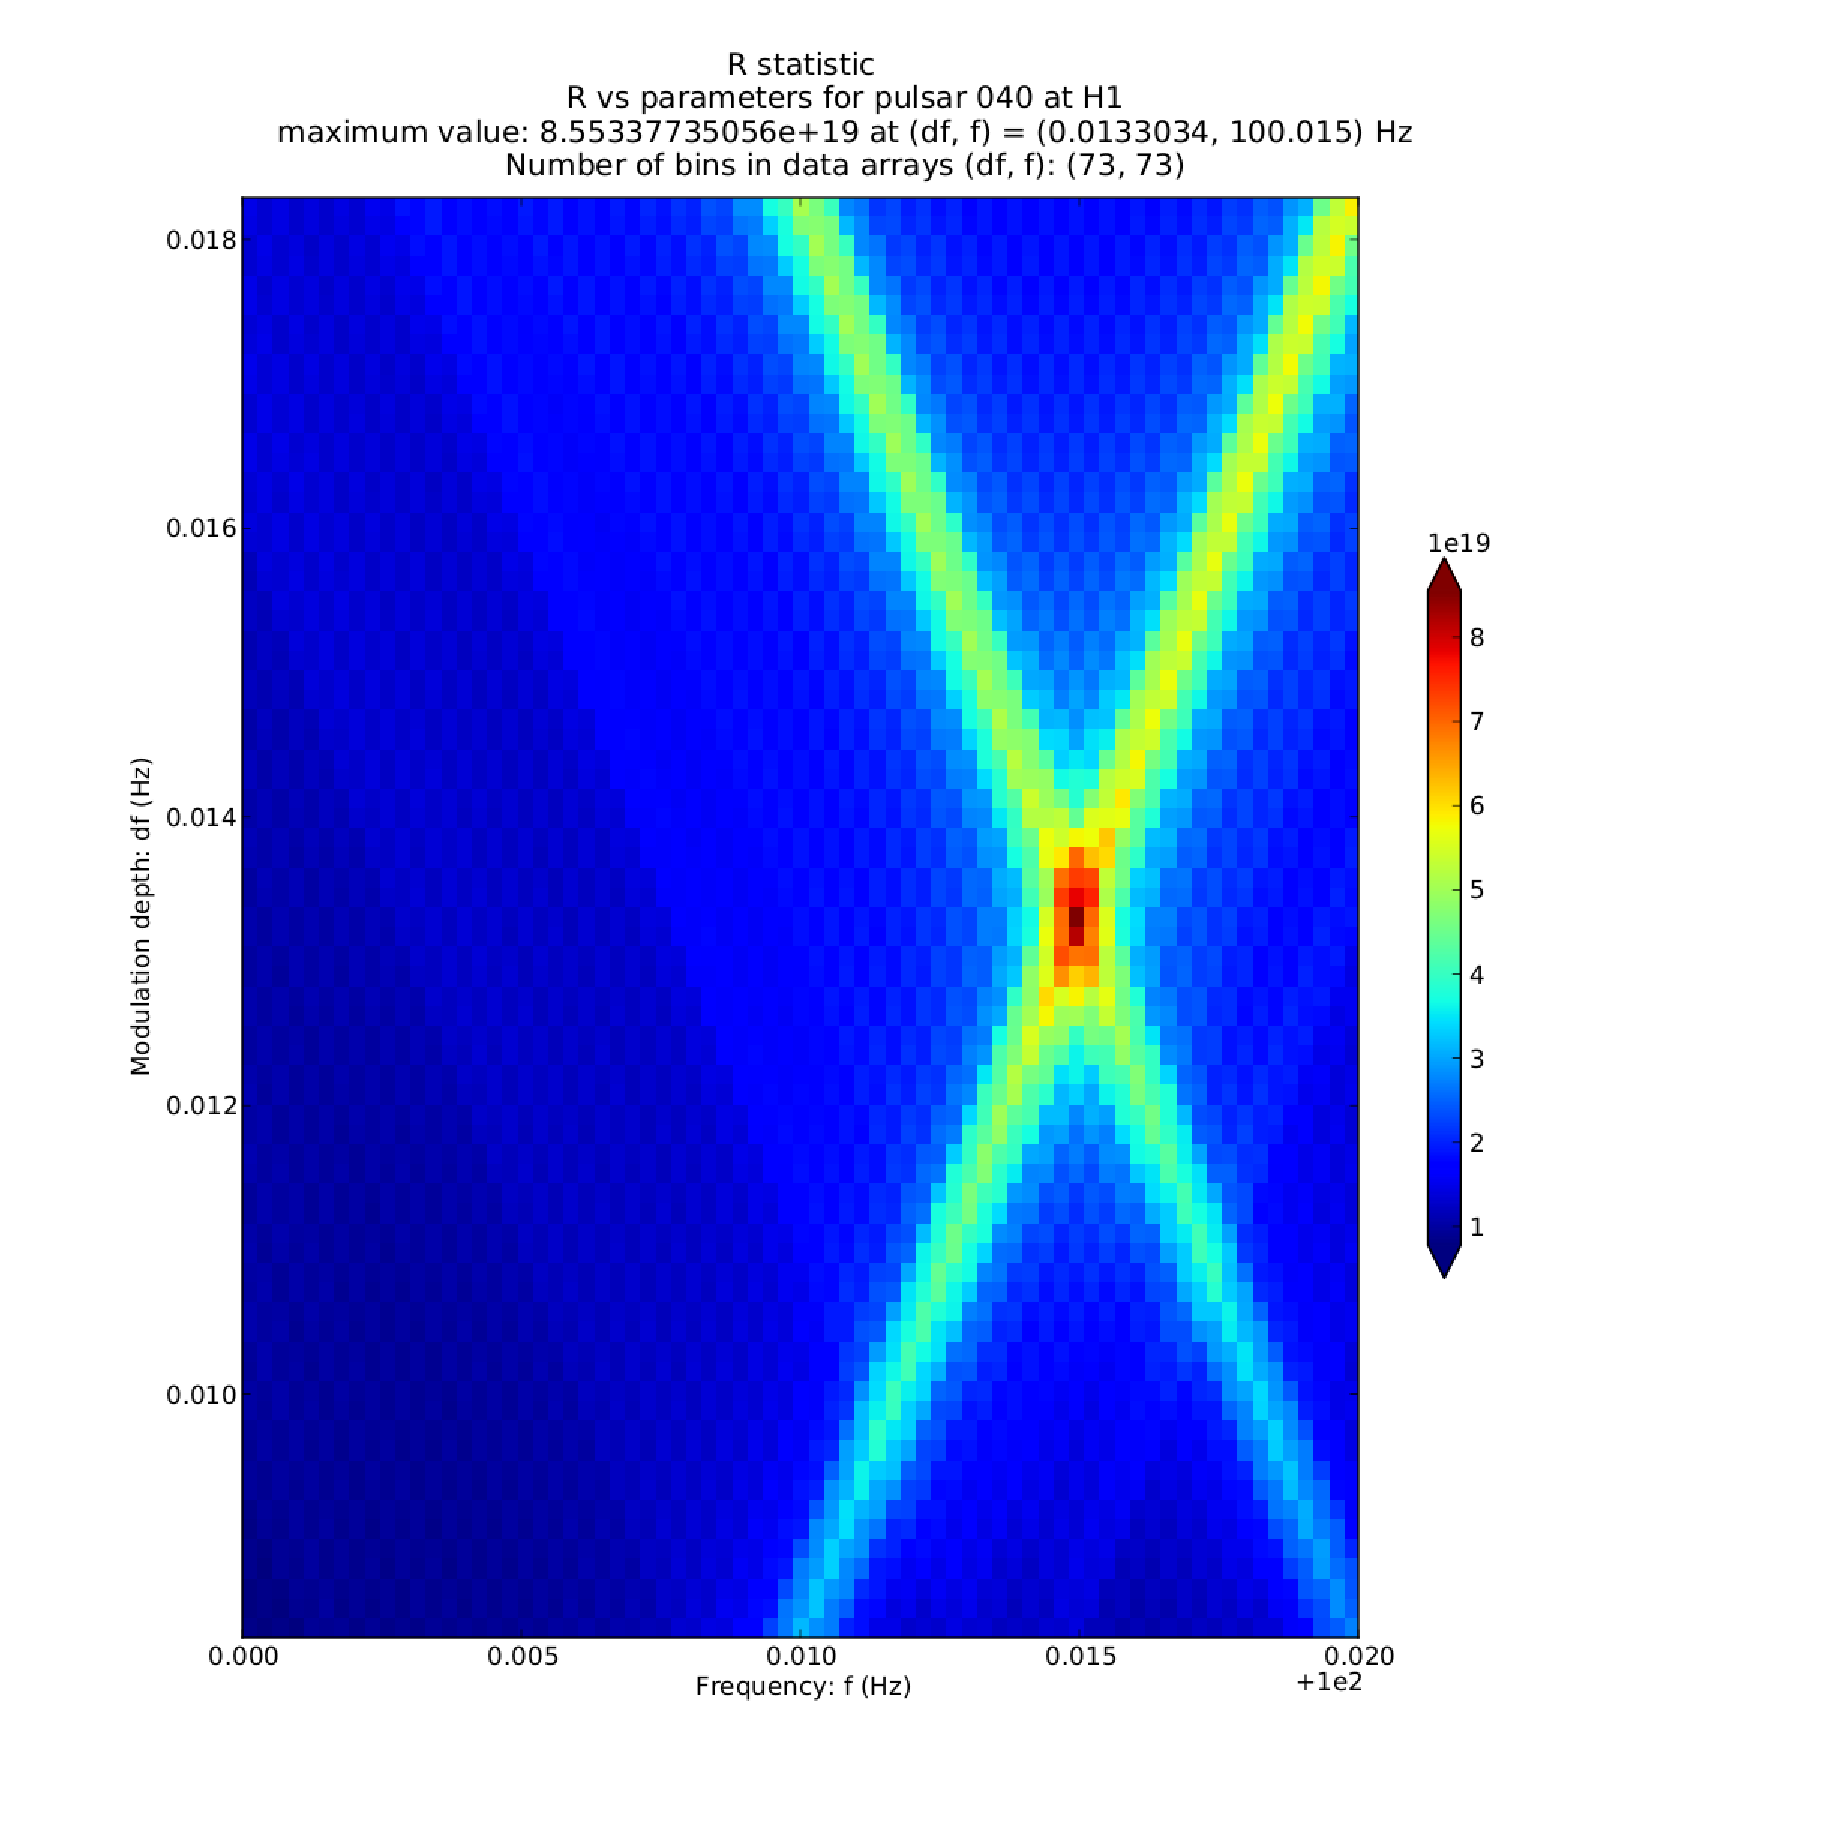
\includegraphics[trim=20 20 20 80, clip, keepaspectratio,height=0.55\paperheight]{plots/R-4e21-on-4e24.eps}
\caption{Signal templates applied to pixels in the $f$-$f'$ plane give $R$ statistics for a simulated pulsar 
%(note: not the same as pulsar $40$ in the Scorpius X-1 mock data challenge) 
at 100.015 Hz and $a \sin i = 1.44$ s. Resulting $R$ values are heatmap-plotted on the $\Delta f$ vs $f$ plane.}
\label{inj_R_statistic}
\end{center}
\end{figure}

\begin{figure}
\begin{center}
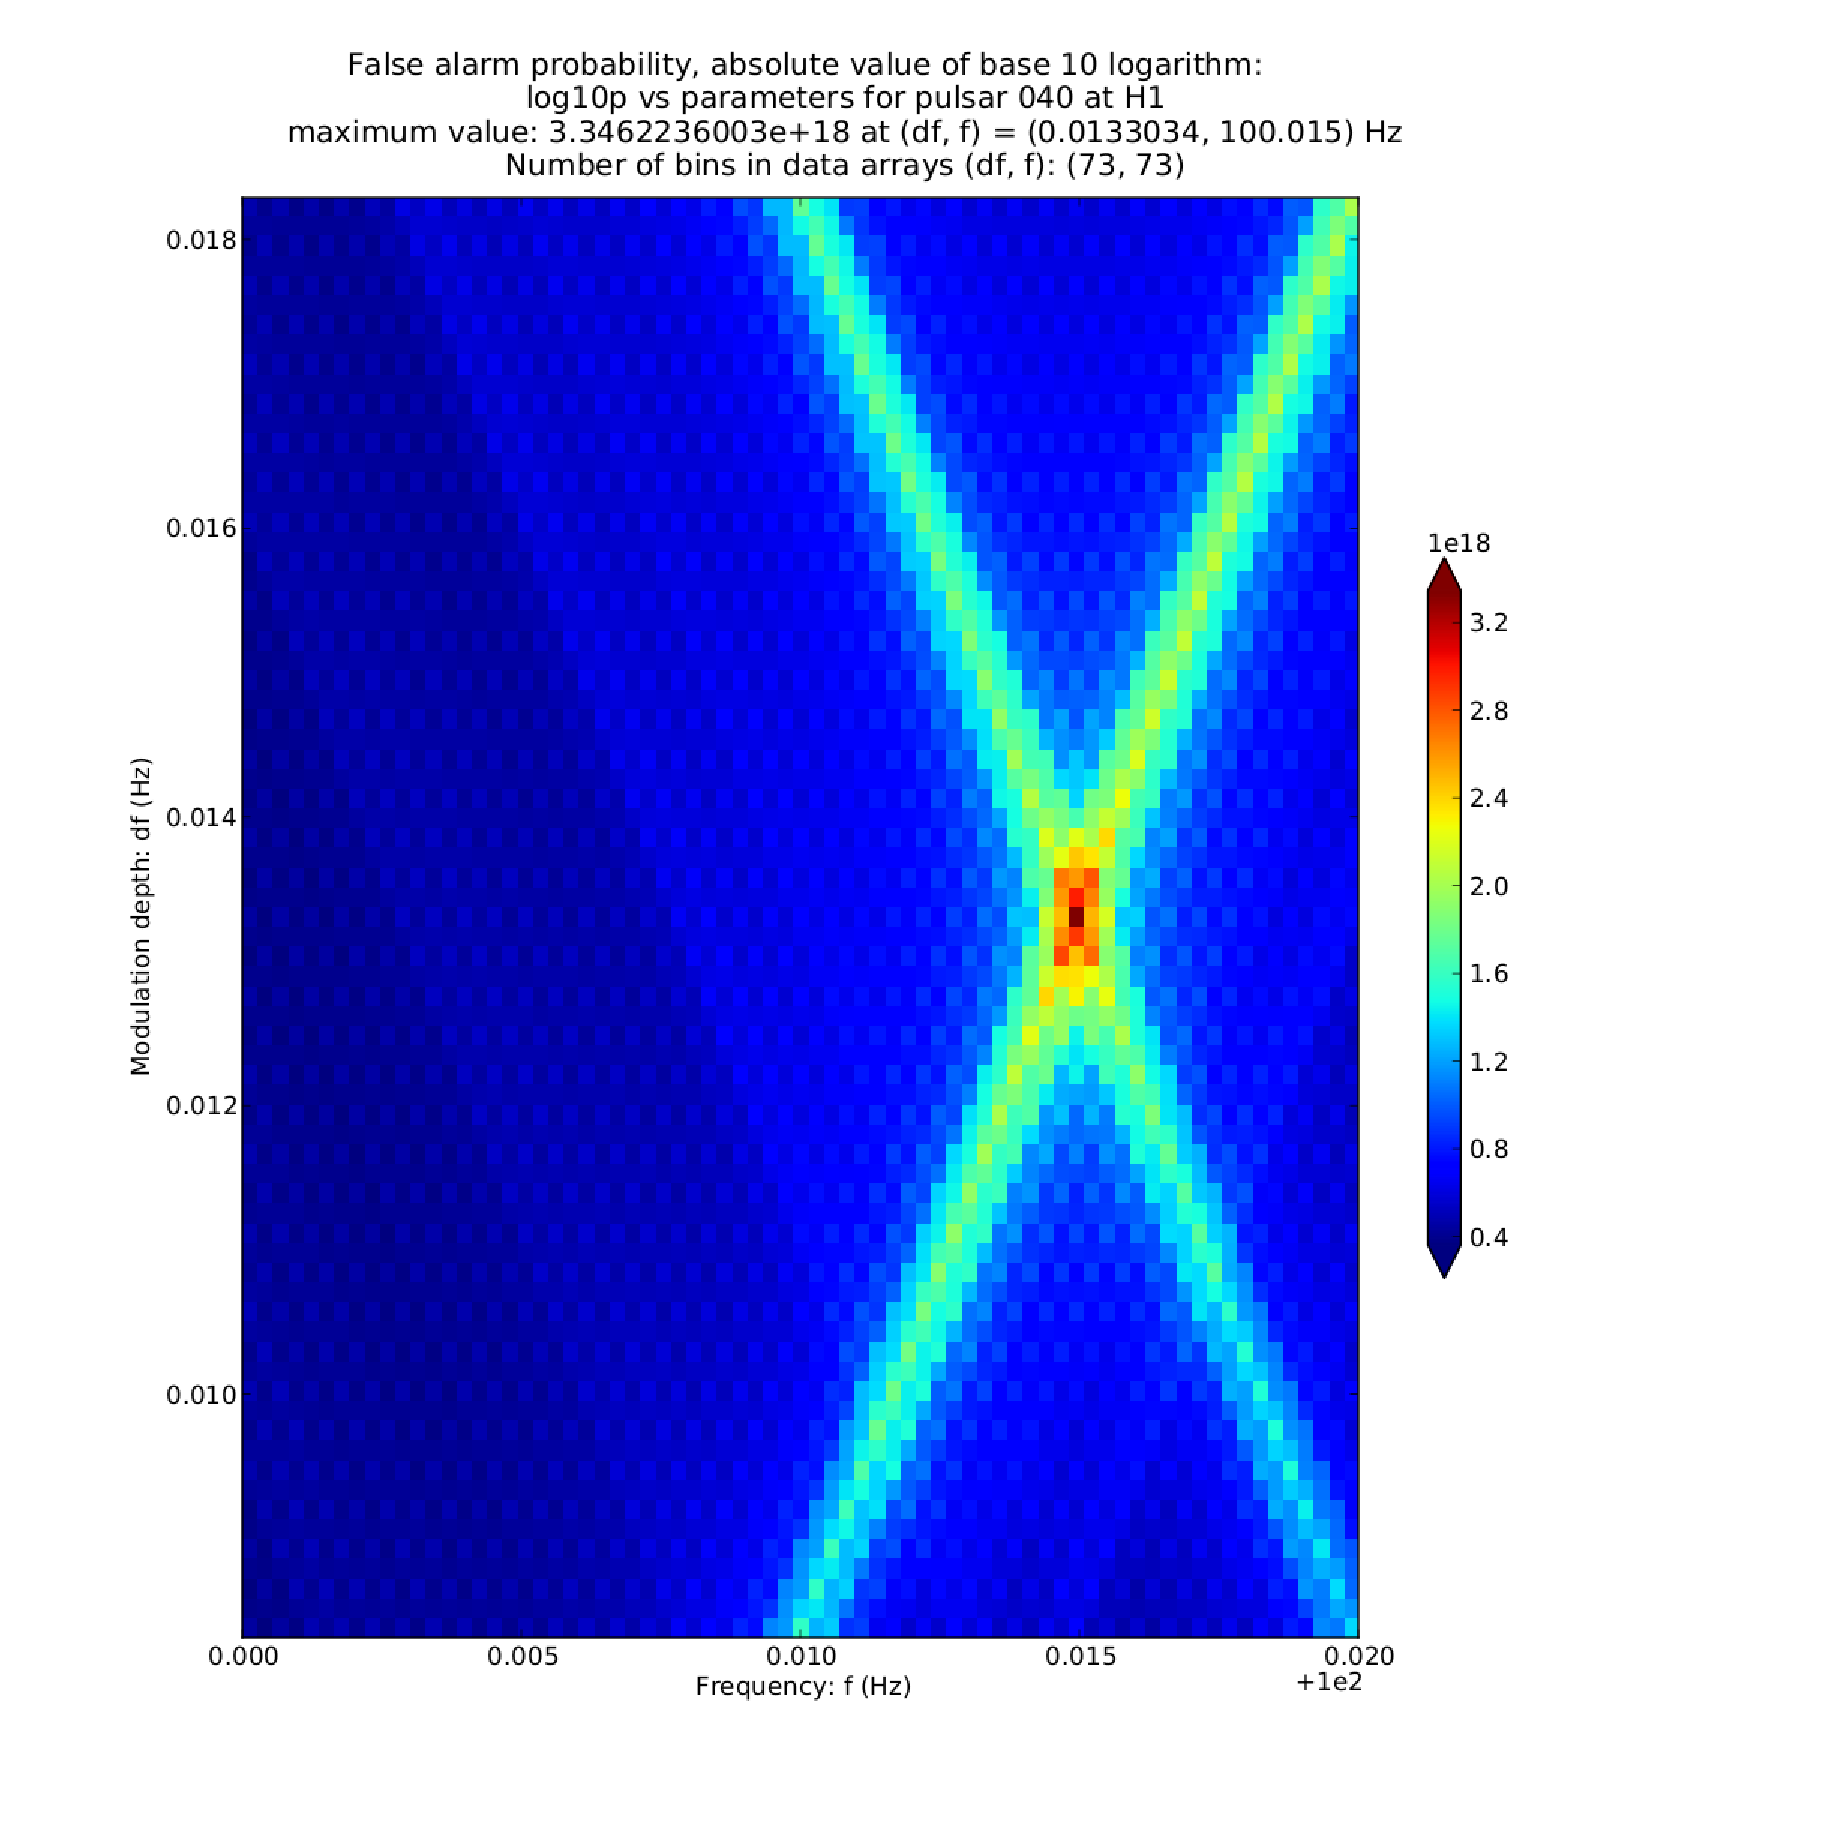
\includegraphics[trim=20 20 20 80, clip, keepaspectratio,height=0.55\paperheight]{plots/Prob-4e21-on-4e24.eps}
\caption{Davies' algorithm translates $R$ statistics into (single-template) $p$-values, plotted on the $\Delta f$ vs $f$ plane.}
\label{inj_log10p}
\end{center}
\end{figure}

\subsection{Template spacing and search metrics}

Searches are conducted by testing a recorded data set using templates corresponding to a putative GW signal.
Many templates are needed, depending on the scale of the search~\cite{GoetzTwoSpectMethods2011}, to cover the range of possible parameters $\theta$.
In the all-sky search, parameters include orbital period $P$ and sky location $(\alpha, \delta)$, but the directed search described herein can be used when these are known, so the parameter space is restricted to frequency $f$ and projected semi-major axis $a \sin i$.
The parameter space grid must be sampled densely enough to constrain $R$-statistic mismatch $\mu \leq 0.2$.
Mismatch is defined by the fractional difference between the $R$ statistic at the true parameters of the signal, $R(\theta_{GW})$, from the maximum $R(\theta)$ obtained; the statistic is designed so that idealy $R(\theta_{GW}) \geq R(\theta)$ for all $\theta$, assuming one signal is present.
Prior simulations have shown that, when $P$ and $(\alpha,\delta)$ are fixed, the $f$ and $a \sin i$ grids are uniform.
Frequency $f$ spacing of $1/2T_\mathrm{SFT}$ is sufficient, and $a \sin i$ is chosen such that modulation depth $\Delta f_\mathrm{obs}$ is spaced at $1/4T_\mathrm{SFT}$.
For a fuller analysis, one can calculate the statistical mismatch metric~\cite{Brady1998}, $g_{ij}$.
Fixed grid spacing corresponds to a flat mismatch metric.

\section*{References}
\bibliographystyle{jphysicsB}
\bibliography{bibliography}

%\section*{Extraneous material for technical notes}
\textbf{REMOVE FROM FINAL PAPER:}
\textit{intended for technical notes in internal use}

\begin{figure}
\begin{center}
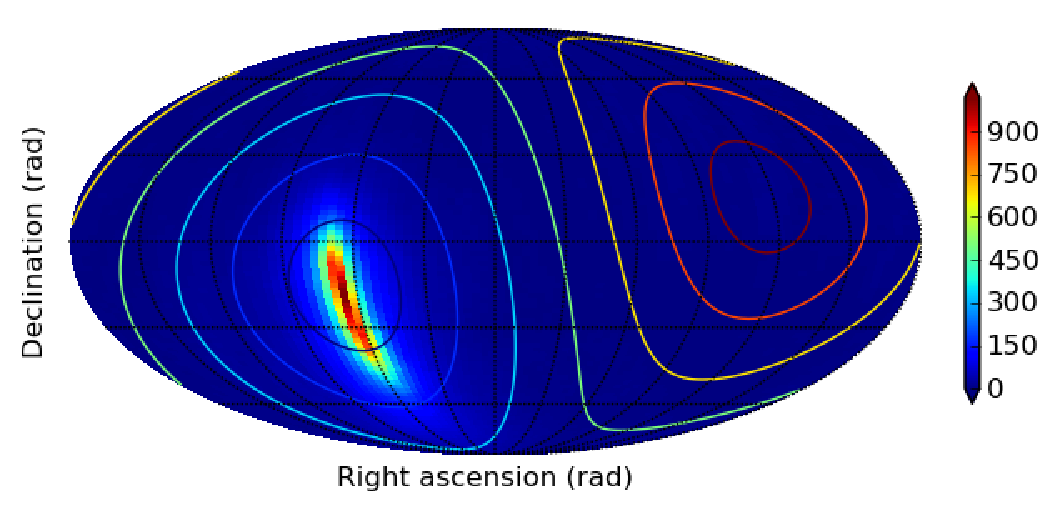
\includegraphics[width=0.6\paperwidth,height=0.2\paperheight]{plots/maptrueH1.eps}
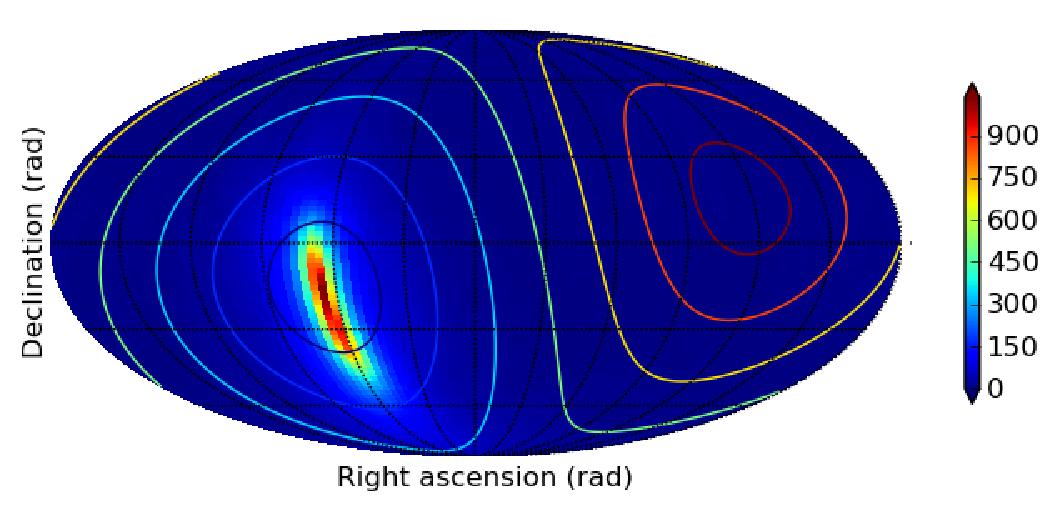
\includegraphics[width=0.6\paperwidth,height=0.2\paperheight]{plots/maptrueL1.eps}
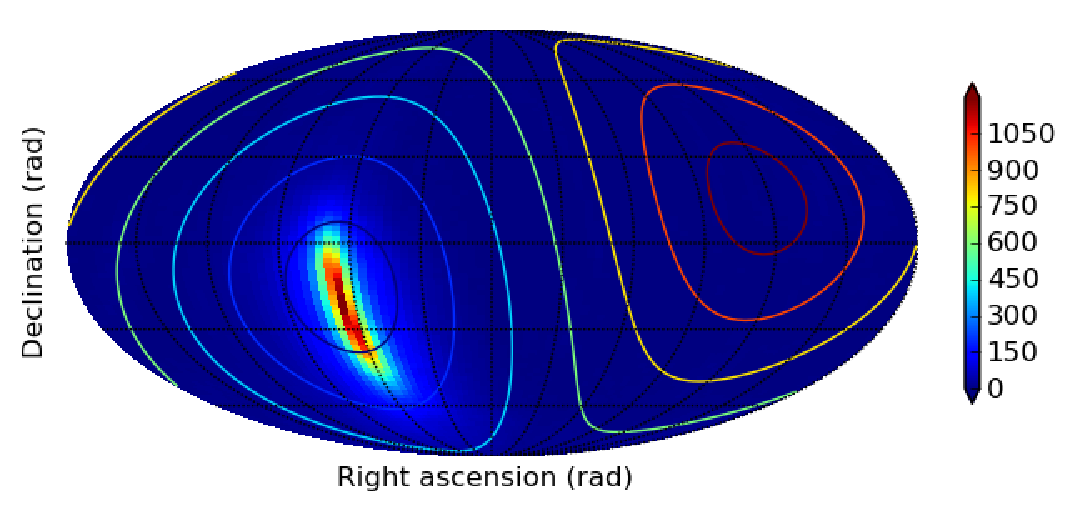
\includegraphics[width=0.6\paperwidth,height=0.2\paperheight]{plots/maptrueV1.eps}
\caption{ All-sky maps (from top to bottom: H1, L1, V1) showing analysis across varying right ascension and declination. 
Scorpius X-1 mock data challenge pulsar 16 (101x101 templates), showing $-\log_{10}p$-value on a Mollweide projection.
Contour lines at 1-radian great-circle distance intervals from the simulated location of Sco X-1.
}
\label{scox1-allsky-maps}
\end{center}
\end{figure}


\begin{figure}
\begin{center}
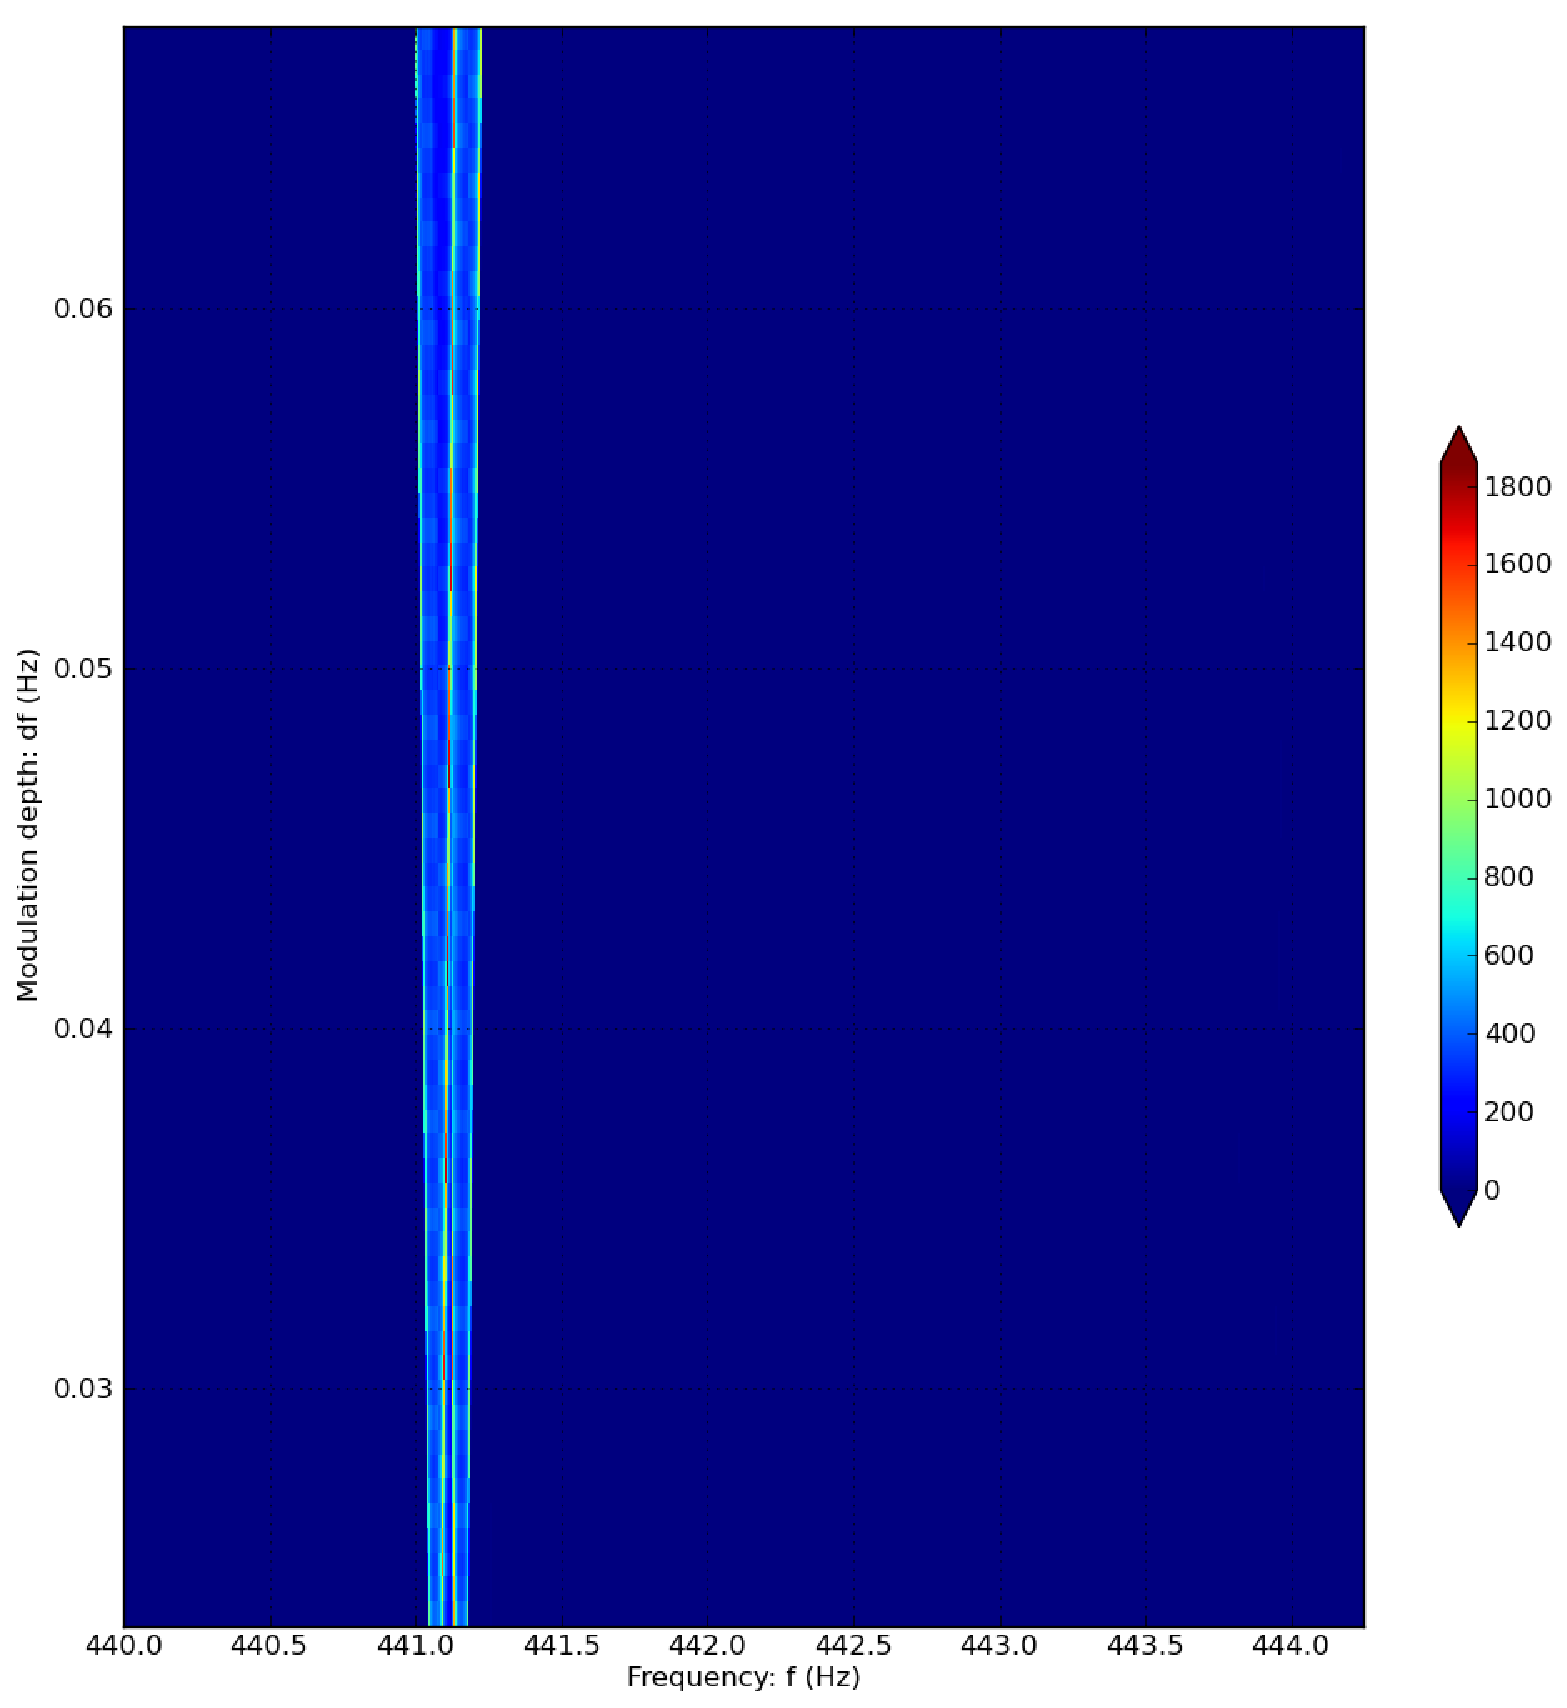
\includegraphics[width=0.65\paperwidth,height=0.5\paperheight]{plots/bandH1-bold.eps}
\caption{
Scorpius X-1 Mock Data Challenge (MDC) pulsar 40 \{H1\}: 5 Hz band. 
The $-\log_{10}p$-value (single-template, applying Davies' Method to the $R$ statistic) is shown in this heatmap, peak in red. 
All templates are plotted on the (frequency, modulation depth) plane.
This is a relatively broadband view.
}
\label{scox1-wide-heatmap-040}
\end{center}
\end{figure}


Figure~\ref{scox1-wide-heatmap-040} shows the result of a 5 Hz-wide analysis on an easily detectable pulsar.

\begin{figure}
\begin{center}
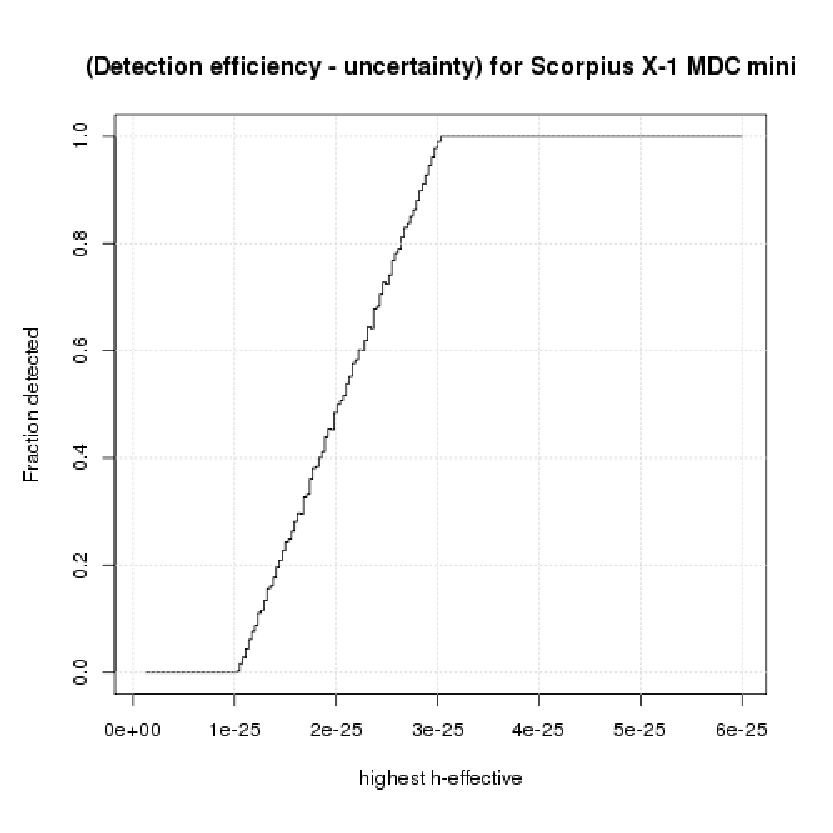
\includegraphics[trim=0 10 10 5, clip, width=0.70\paperwidth,height=0.48\paperheight]{plots/PlotHeffDistH0DetectionEfficiency200breaks.eps}
\caption{ Simulated detection efficiency curve. Because the $\cos \iota$ ambiguity simulation require a priori model of detection efficiency, we describe it simply. Here, no detections are claimed below $1\times 10^{-25}$, all are detected above $3\times 10^{-25}$, and the probability of detection rises uniformly on the intervening interval.
\label{fig:plotheffdisth0detectionefficiency200breaks}}
\end{center}
\end{figure}

\subsection{Sensitivity depth}
\label{sensitivity-depth-appendix}

Sensitivity depth answers whether an analyses has the power to see a certain strain in detector data.
GW observatory data has an amplitude spectral density, $S_H^{1/2}(f)$.
The minimum $S_H^{1/2}(f)$ was about $2\times 10^{-23}\mathrm{~Hz}^{-1/2}$ in initial LIGO or $4\times 10^{-24}$ $\mathrm{~Hz}^{-1/2}$ in Advanced LIGO~\cite{HarryALIGO2010}, which should be achieved in the 100-300 Hz band.
%Coherent searches are the most sensitive in terms of \textit{sensitivity depth}, or power to resolve signals for a given noise spectral sensitivity.
Define the depth as $D$,

\begin{equation}
D(f) \equiv \frac{S_H^{1/2}(f)}{h_0(f)},
\end{equation}

\noindent for an $h_0(f)$ at a specified confidence level and frequency.
In LIGO S4 data, the Hough, StackSlide, and PowerFlux methods achieved 95\%-confidence upper limits on $h_0$ of approximately $4.3\times 10^{-24}$,
% in noise of $2.5 \times 10^{-19} \mathrm{~m~Hz}^{-1/2}$, 
or $6.25\times 10^{-23} \mathrm{~Hz}^{-1/2}$,
a sensitivity depth of about 15$\mathrm{~Hz}^{-1/2}$,
and improvements have been made since this comparison~\cite{LSCPulsarS4}.
Complications for coherent searches, such as spin-wandering, unknown orbital parameters, and sky location, motivated the development of TwoSpect.
In the all-sky search of S6 data~\cite{GoetzTwoSpectResults2014}, the most constraining 95\%-confidence upper limit of $2.3\times10^{-24}$ (assuming circularly-polarized GW) was achieved in a detector noise floor around $2\times 10^{-23} \mathrm{~Hz}^{-1/2}$~\cite{Fricke2009}, implying a sensitivity depth around 10$\mathrm{~Hz}^{-1/2}$ for circular polarization.
Searching for unknown sources across the sky is justified: GWs theoretically less directional than beamed X-ray flux, so sources with GW luminosity equal or greater than Sco X-1 might be as-yet unknown in electromagnetic counterparts.
Yet the all-sky search~\cite{GoetzTwoSpectMethods2011} parameter space is too large to search at full sensitivity.
Sco X-1, conversely, allows a directed search at its sky location, projected semi-major axis and orbital period.
Fully template-testing the reduced parameter space is intended to yield enhanced sensitivity depth.


    \subsection{Signal model}
    \label{signal-model-appendix}

%\textbf{Signal model}\\

Gravitational waves from a neutron star in a binary system are described by strain as a function of time $h_0(t) = h_0 e^{i \Phi(t)}$. 
Measured strain $h(t)$ depends on the detector response to $h_0(t)$.
Amplitude $h_0$ depends on the astrophysical parameters of the neutron star~\cite{Jaranowski1998}.
The phase model $\Phi$ can be described using detector time $t$ and Solar System Barycenter (SSB) time $t_\mathrm{SSB}$.
Travel from the source to SSB introduces an overall phase shift; uncertainty in the distance and proper motion is systematic and the same for gravitational and electromagnetic observations.
Detector time is recorded in GPS time, running parallel with Terrestrial Time (TT), and SSB time runs parallel with Barycentric Dynamical Time (TDB). 
SSB time corrects $t$ by $\delta t_R$ for relativistic effects.
Another overall phase shift is caused by  Roemer delay $\Delta t_R$, the dot product of $\hat{n}/c$ from the SSB to the sky location of interest with $\vec{r}$ from the SSB to the detector~\cite{Jaranowski1998,GoetzTwoSpectMethods2011,TwoSpectCoherentGoetz2015}.
Barycentering detector-frame data is equivalent to resampling in $\tau(t) = t_\mathrm{SSB}(t) + \Delta t_R(t)$, 

% OLD STUFF BELOW
%The phase model $\Phi$ can be described using detector time $t$ and Solar System Barycenter (SSB) time $t_\mathrm{SSB}$.
%The Lorentz dilation is $\gamma= \sqrt{1+(v/c)^2}\approx 5\times 10^{-9}$ for the Earth's motion.
%Gravitational time dilation is $\sqrt{1-2GM/(rc^2)}$ and of comparable magnitude with opposite sign. 

\begin{equation}
\tau(t) 
% &= \gamma + \Delta t_R, \\ 
 = t + \frac{\vec{r}(t) \cdot \hat{n}}{c} + \delta t_R.
\label{barycentering_time_domain}
\end{equation}

Binary motion can be described as modulating GW emission frequency $f=f_0$ by the orbital motion of the companion object~\cite{GoetzTwoSpectResults2014}.
The frequency $f$ is usually presumed equal to $2\nu_s$ for a neutron star spin frequency of $\nu_s$, as it would be for quadrupolar radiation due to ellipticity on the star.
Orbital modulation occurs at a frequency $\Omega = 2\pi/P$ with a frequency modulation depth $\Delta f_\mathrm{obs}$,

\begin{equation}
\Delta f_\mathrm{obs} = \frac{2 \pi f_0 \cdot (a \sin i)}{cP}.
\label{TwoSpect_mod_depth}
\end{equation}

\noindent The binary system's projected semi-major axis is $a \sin i$, inclined by the angle $i$ of the orbital axis measured with respect to the observer's line-of-sight; $P$ is the orbital period of the system.
It is useful to express $a \sin i$ in light-seconds.
Orbital phase is specified by $T_\mathrm{asc}$, the SSB time of ascension, when the companion object crosses the ascending node; the phase can nevertheless be stated as a function of detector time $t$.
Future work may consider eccentricity $e$, but it was considered small enough to not be simulated in our comparison~\cite{ScoX1MDC2015PRD}.
Reference time is established by $\Phi(T_\mathrm{ref}) = \Phi_0$.
An unknown spin-wandering term, $\delta \Phi_\mathrm{spin-wander}$, is hypothesized.

Phase $\Phi$ can thus be expressed in $t$, using $\tau_B$ to resample the binary motion: 

\begin{equation}
\tau_B(t) \equiv \tau(t) + [a \sin(i)/c] \sin (\Omega [t - T_\mathrm{asc}]),
\label{resampled_time}
\end{equation}
\begin{eqnarray}
\Phi(t) 
    &= \Phi_0 &+ \delta \Phi_\mathrm{spin-wander} + 2\pi f_0 \cdot \left(\tau_B(t) - T_\mathrm{ref}\right), \label{compact_phase_model} \\
    &= \Phi_0 &+ \delta \Phi_\mathrm{spin-wander} \nonumber\\
    & &+ 2\pi \left[f_0 \cdot \left(\tau(t)-T_\mathrm{ref}\right) + \frac{\Delta f_\mathrm{obs}}{\Omega} \sin (\Omega [t - T_\mathrm{asc}]) \right], \\
    &= \Phi_0 &+ \delta \Phi_\mathrm{spin-wander} \nonumber\\
    & &+2\pi \left[f_0 \cdot \left(t + \frac{\vec{r}(t)\cdot \hat{n}}{c}+\delta t_R-T_\mathrm{ref}\right)\right] \nonumber\\
    & &+2\pi \left[ \frac{\Delta f_\mathrm{obs}}{\Omega} \sin (\Omega [t - T_\mathrm{asc}]) \right].
\label{phase_model}
\end{eqnarray}


Strain as a function of time, $h(t)$, is expected to be present in two polarizations, \textit{plus}, $h_+$, and \textit{cross}, $h_\times$.
Our analyses uses $h(t)$ from a single detector that responds to both polarizations, depending on right ascension $\alpha$, declination $\delta$, time $t$ and polarization angle $\psi$, with functions $F_+$ and $F_\times$.
The $F_+$ and $F_\times$ also depend on detector geographical location and orientation.
The proportion of the signal in each polarization is determined by the polarization angle $\iota$ of the neutron star rotation axis with respect to the line of sight of the observer.
Antenna-pattern response is calculated by projecting the polarization tensor, for $\psi$ and sky location, onto the detector~\cite{YunesSiemens2013}.
Antenna response is represented by the covector $F_j$ with components $(F_+, F_\times)$:

\begin{eqnarray}
F_j(t,\alpha,\delta,\psi) 
%\equiv 
%\left( \begin{array}{rr} F_+(t, \alpha, \delta, \psi)  & F_\times(t, \alpha, \delta, \psi) \end{array} \right) \nonumber \\
=
\left( \begin{array}{rr} \cos 2 \psi & \sin 2 \psi \end{array} \right) \left( \begin{array}{cc} a(t, \alpha, \delta) & b(t, \alpha, \delta) \\ b(t, \alpha, \delta) & -a(t, \alpha, \delta) \end{array}\right)   ,
\end{eqnarray}

\noindent where detector specific responses $a$ and $b$ depend on ($\alpha,\delta$) and location~\cite{Jaranowski1998}. Incident GW polarization is $\iota^j_k J^k$, acting on the Jones vector $J^k$:
%
%\begin{equation} 
%\textbf{h}_j = h_0 (\iota_{jk} \Phi_k),
%\end{equation}
%
%\noindent where
%
\begin{eqnarray}
\iota^j_k =
\left(
\begin{array}{cc}
\frac{1+\cos^2 \iota}{2} & 0 \\
0 & \cos \iota \\
\end{array}
\right),\\
J^k = \left(
\begin{array}{c}
1\\
-i\\
\end{array}
\right).
\end{eqnarray}

\noindent The phases of the two polarizations are expressed by the vector $\Phi^k(t)$:

\begin{eqnarray}
\Phi^k(t) =
\Re\left[J^k e^{\mathrm{i} \Phi(t)} \right]
=
\left(
\begin{array}{c}
\cos \Phi(t)\\
\sin \Phi(t)\\
\end{array}
\right).
\end{eqnarray}

\noindent It is convenient to factorize $\mathcal{A}_k \equiv h_0 \cdot (F_j \iota^j_k)$~\cite{TwoSpectCoherentGoetz2015} and to introduce $A \equiv (\mathcal{A}_+ - \mathrm{i} \mathcal{A}_\times )/2$. 
Note $A = (1/2)h_0 \cdot (F_j \iota^j_k J^k)$. 
Complex conjugate $*$ yields a compact waveform expression.
Gathering terms, the expected GW strain model is $h(t)$:

\begin{eqnarray}
h(t)
 &= \mathcal{A}_k \Phi^k, \\
 &= \Re\left[h_0 F_j \iota^j_k J^k e^{\mathrm{i}\Phi(t)}\right], \\
  &= A e^{\mathrm{i}\Phi(t)} + A^* e^{-\mathrm{i}\Phi(t)}, \label{Evan_expression_ht}\\
%h(t) 
&= h_0 F_+ \frac{1+\cos^2 \iota}{2}\cos \Phi(t) +
  h_0 F_\times \cos \iota \sin \Phi(t).
\label{amplitude_model}
\end{eqnarray}

\noindent Circular polarization, when $\cos \iota =1$, maximizes $h(t)$, though $\iota$ is often unknown.

%Although one can interpret $F_j$, $\iota^j_k$, and $\Phi^k$ in several ways, the core 
Searches for $h(t)$ can model $\Phi(t)$, where $\iota$ and $\psi$ are often nuisance parameters and the strain amplitude $h_0$ is later inferred.
The response $F_j$ decomposes to a unit-vector right-multiplied by the (transverse-traceless) detector response matrix. 
This detector matrix can be interpreted as a metric for the inner product $h(t)$ of the polarization tensor and the Jones vector.
We compose $F_j$ with the (diagonal) dilation-rotation $\iota^j_k$ to produce $A$.
Equation~\ref{Evan_expression_ht} illustrates that $A$ is half the modulus, and $\Phi$ the argument, of $h(t)$; this formalism generalizes to include multiple detectors~\cite{TwoSpectCoherentGoetz2015}. 
The measured output $x(t)$ of a detector corresponds to the signal $h(t)$ plus noise $n(t)$,

\begin{equation}
x(t) = h(t) + n(t).
\end{equation}

        \subsection{TwoSpect statistics}
        \label{all-sky}

The TwoSpect program calculates a test statistic $R$ and single-template $p$-value for a putative template waveform of a neutron star emitting continuous GWs in a binary system.
The construction of this $R$-statistic can be described in several steps.
Science/observing runs are first parcelled into overlapping short Fourier transforms (SFTs), performed in the detector frame.
The SFTs have typical coherence time $T_\mathrm{SFT}$, also referred to as $T_\mathrm{coh}$ in past work, ranging from 60 s to 1800 s, depending on the hypothesized time-derivative of neutron star frequency~\cite{GoetzTwoSpectMethods2011}.
The total number of SFTs with 50\%-overlap for an observing time $T_\mathrm{obs}$ is $N$,

\begin{equation}
N = \mathrm{floor}\left(\frac{2 T_\mathrm{obs}}{T_\mathrm{SFT}}\right) - 1.
\end{equation}

\noindent SFT number in the observing run are indexed by $n \in [0,\ldots,N-1]$; SFT frequency bin is indexed by $k \in [0,\ldots,K -1]$, where $K = T_\mathrm{SFT} f_N$ for a Nyquist frequency $f_N$ and only positive frequencies $k = T_\mathrm{SFT} f$ are used. 
Thus the transformation from time series to SFTs is a map from $x(t)$ (containing $h(t)$) to $\tilde{x}^n_k$.

Each SFT frequency bin $\tilde{x}^n_k$ is Doppler shifted to a frequency bin in the SSB frame corresponding to the sky location, frequency, and time $t$ of the midpoint of the SFT $n$ under investigation: $k(f(\alpha,\delta,t)) \rightarrow k(f_\mathrm{SSB}(\tau))$.
This barycentering procedure corresponds to the time-domain Equation~\ref{barycentering_time_domain}.
Figure~\ref{tfplane-figure}
shows a simulated signal in the resulting time-frequency plane.
Henceforth, barycentering is implicit in the $k$ index.
Define the power $P^n_k = 2|\tilde{x}^n_k|^2/T_\mathrm{SFT}$.
Let $\left<P_k\right>^n$ be the expected (estimated from a running mean over nearby $n$) noise-only power in a frequency bin $k$ for SFT $n$.
Also let $F^2_n \equiv F_{+,n}^2 + F_{\times,n}^2$ for the antenna pattern at the chosen sky location and SFT $n$ -- taking this equal-weighted sum implies an assumption of circular polarization. 
Then the estimated power in a given bin $\tilde{P}^n_k$ is normalized such that random, white, Gaussian noise will have an expectation value of 1~\cite{GoetzTwoSpectMethods2011}:

\begin{equation}
\tilde{P}^n_k = \frac{F_n^2 (P_k^n - \left<P_k\right>^n)}{(\left<P_k\right>^n)^2}\left[\sum\limits_{n'}^N \frac{F_{n'}^4}{(\left<P_k\right>^{n'})^2} \right]^{-1}.
\label{equation_with_antenna_pattern}
\end{equation}

Then each row of barycentered frequency bins $k$ is treated as a time series in $n$.
Power for bin $k$ in that time series is Fourier transformed by $\mathcal{F}_{f'}$ into $Z_k(f')$ (Figure~\ref{ffplane-figure}), where $f'$ is the second Fourier transform frequency.
During the transform, the background noise power $\lambda(f')$ is estimated from the noise in the SFTs, assuming the noise is Gaussian.
This second Fourier power $Z_k(f')$ follows a $\chi^2$ distribution with 2 degrees of freedom and mean 1.0, is proportional to $h^4$, and is constructed by 

\begin{equation}
Z_k(f') = \frac{\left| \mathcal{F}_{f'} [\tilde{P}^n_k]  \right|^2}{\left< \lambda(f') \right>}.
\label{second_Fourier_power}
\end{equation}

At this point it is helpful to explicitly define how the background is constructed.
An average noise ratio per frequency bin, $\rho_k$, is defined by

\begin{equation}
\rho_k = \frac{\sum_{n=0}^{N-1} \left(\left<P_k\right>^n\right)^{-1}}{\sum_{n=0}^{N-1} \left(\left<P_k\right>^n\right)^{-2}} \left(\frac{1}{K} \sum_{k=0}^{K-1} \sum_{n=0}^{N-1} \left(\left<P_k\right>^n\right)^{-1} \right).
\end{equation}

\noindent Designate the median, over $k$, of $\left<P_k\right>^n$ as $\mu_n$.
A random variable $Y$, drawn from an exponential distribution according to $\mu_n$ and used to construct a simulated time-frequency power $X_n$:

\begin{equation}
X_n(Y_q) = \left(\frac{(Y_q)}{\mu_n} - 1 \right) \times \frac{F_n^2}{\mu_n} \left[ \sum\limits_{n'=0}^{N-1} \frac{F_{n'}^4}{(\mu_{n'})^2} \right].
\end{equation}

\noindent We then compute the average noise in each of $F' = (\mathrm{floor}(N/2) +1)$ second-frequency bins $f'$.
A Monte Carlo simulation with $T$ trials, typically 4000, generates the random variable $Y$.
The $Y$ are indexed by trial $q$.  
The simulation computes the un-normalized average noise $\lambda(f')$, with mean $\left< \lambda(f') \right>$:

\begin{eqnarray}
\lambda(f') = \frac{1}{T} \sum_{q=0}^{T-1}|\mathcal{F}_{f'}\left(X_n (Y_q)\right)|^2.
\end{eqnarray}

\noindent The background power of a pixel, used later in constructing test-statistics, is $\lambda_k(f')$:

\begin{equation}
\lambda_k(f') = \rho_k \frac{\lambda(f')}{\left< \lambda(f') \right>}.
\end{equation}

Signal templates encode the expected $h(t)$ into pixel weights $w$. 
Weights are applied to pixels on the frequency-prime $f'$ vs frequency $f$ plane to give the test statistic $R$; the directed search uses templates defined in the $f$ vs $t$ plane by $x$, then Fourier-transformed into $w$. 
A template has a requested length, $M$, and pixels are indexed by $i \in [0,M-1]$ pixels such that $w_0$ is largest and $w_i \geq w_{i+1}$.
Weights are normalized such that the sum of $w_i$ equals one.
The exact templates depend on SFT number $n$, frequency bin $k$ corresponding to $f_0$, frequency bin $z$ of interest, and SFT coherence time midpoint $T_m$.

Calculating the templates involves Taylor expansion for the coherence time of an SFT, then Fourier transforming a sampled time series.
A dot denotes $d/dt$.
Let $t_B \equiv t + [a \sin (i)/c]\sin(\Omega[t-T_\mathrm{asc}])$, so $\dot{t}_B = 1 + [\Delta f_\mathrm{obs}/f] \cos(\Omega [t_m-T_\mathrm{asc}])$.
Then $\dot{\tau}_B = \dot{t}_B + \frac{d}{dt}(\Delta t_R +\delta t_R)$.
Expand $\Phi(t_m)$ from Equation~\ref{compact_phase_model} about $t_m$:

\begin{equation}
\dot{\tau}_B = 1 + \frac{\vec{v}(t_m) \cdot \hat{n}}{c} + \frac{d}{dt}\delta t_R+ \frac{\Delta f_\mathrm{obs}}{f_0} \cos \left(\Omega [t - T_\mathrm{asc}]\right),
\label{tau-time-derivative}
\end{equation}
\begin{eqnarray}
\Phi(t_m) &\approx \Phi_0 &+ \delta \Phi_\mathrm{spin-wander} \nonumber \\
  & &+ 2 \pi f_0 \left(t_m + \frac{\vec{r}(t_m)\cdot \hat{n}}{c} +\delta t_R- T_\mathrm{ref} + \dot{\tau}_B \cdot [t-t_m] \right). 
\end{eqnarray}

\noindent Indexing $L = 2f_\mathrm{Nyquist}T_\mathrm{SFT}$ time samples by $l\in [0,\ldots,L-1]$, we can gather constant terms into $\hat{\Phi}$.
Then take the Fourier transform $\tilde{h}_k \equiv \mathcal{F}_k(h(t))$ of positive frequencies in the signal model, Equation~\ref{Evan_expression_ht}, allowing windowing weights $u_l$ with $C\equiv\left(\sum_{l=0}^{L-1} u_l^2 / L \right)^{1/2}$:

\begin{eqnarray} 
\hat{\Phi} &\equiv \Phi_0 &+ \delta\Phi_\mathrm{spin-wander} \nonumber\\
  & &+ 2\pi f_0 \left(t_m + \frac{\vec{r}(t_m)\cdot\hat{n}}{c} +\delta t_R- T_\mathrm{ref} - \dot{\tau}_B t_m\right),
\end{eqnarray}
\begin{eqnarray}
\tilde{h}_k 
  &= \frac{T_\mathrm{SFT}}{CL} \sum\limits^{L-1}_{l=0} u_l A e^{\mathrm{i} \left(\hat{\Phi} + 2\pi f_0 \dot{\tau}_B [l T_\mathrm{SFT}/L]\right)} e^{- 2\pi \mathrm{i} [lk /L]},\\ 
%  &= \frac{T_\mathrm{SFT}}{CL} \sum\limits^{L-1}_{l=0} u_l A e^{\mathrm{i} \hat{\Phi}} e^{2 \pi \mathrm{i} \left(f_0 \dot{\tau}_B T_\mathrm{SFT} - k\right)l/L},\\
  &= A e^{\mathrm{i} \hat{\Phi}} \frac{T_\mathrm{SFT}}{CL} \sum\limits^{L-1}_{l=0} u_l \left[e^{2\pi \mathrm{i} \left(f_0 \dot{\tau}_B t_\mathrm{SFT} - k\right)/L} \right]^l.
\label{Fourier_transform_of_signal}
\end{eqnarray}

\noindent Equation~\ref{Fourier_transform_of_signal} contains a geometric series that converges in the large $L$ limit to a Dirichlet kernel~\cite{TwoSpectCoherentGoetz2015}.
Defining $\delta_k \equiv \left(f_0 \dot{\tau}_B T_\mathrm{SFT} - k\right)$, the kernel $D_h$ for the typical Hann window, C = $\sqrt{3/8}$, yields the Fourier transform of the signal model precisely:

\begin{equation}
D_h (\delta_k) = \frac{\mathrm{i} e^{2\pi \mathrm{i} \delta_k} - \mathrm{i}}{4\pi \delta_k \left[(\delta_k)^2 - 1 \right]},
\end{equation} 
\begin{equation}
\tilde{h}_k = A e^{\mathrm{i} \hat{\Phi}} \frac{T_\mathrm{SFT}}{C} D_h \left( \delta_k \right).
\end{equation}

\noindent taking the power $|\tilde{h}_k|^2 = \tilde{h}_k^*\tilde{h}_k$, and defining a coefficient $r_{1/2}= h_0^2 \cdot (\mathcal{A}_+^2 + \mathcal{A}_\times^2)\cdot T_\mathrm{SFT}^2$ along with $\mathrm{sinc}(x) \equiv \sin (\pi x)/ (\pi x)$,

\begin{eqnarray}
|\tilde{h}_k|^2 &= \frac{h_0^2}{4} \cdot (\mathcal{A}_+^2 + \mathcal{A}_\times^2)\cdot\frac{T_\mathrm{SFT}^2}{3/8} \left|\frac{2 - 2 \cos(2\pi \delta_k)}{16 \pi^2 \delta_k^2 [\delta_k^2 -1]^2} \right|,\nonumber \\
 &= \frac{r_{1/2}}{4} \frac{2}{3} \frac{\mathrm{sinc}^2\left(\delta_k\right)}{[\left(\delta_k \right)^2-1]^2}.
\label{modern_tfplane_template_power}
\end{eqnarray} 

Equation~\ref{modern_tfplane_template_power}, multiplied by $4$ to normalize for having taken positive frequencies only, corresponds to previous calculations for Hann-windowed power $|x_z(n)|^2$ in a pixel in the time-frequency plane~\cite{GoetzTwoSpectMethods2011}:
%Code is available online~\cite{LALAPPSrepo}.

\begin{equation}
|x_z (n)|^2 = \frac{2}{3} \frac{\mathrm{sinc}^2\left[k + \Delta f_\mathrm{obs} T_\mathrm{SFT} \sin (2\pi n T_m/P) - z \right]}{\left[ (k + \Delta f_\mathrm{obs} T_\mathrm{SFT} \sin (2\pi n T_m / P) - z)^2 - 1 \right]^2},
\label{methods_paper_template_power}
\end{equation}

\noindent where $z$ is now independent instead of $k$, which denotes the bin of the central frequency. 
Substituting $\sin(2\pi nT_m/P) \leftrightarrow \cos(\Omega [t-T_\mathrm{asc}])$ is permitted, because taking the second Fourier power with Equation~\ref{second_Fourier_power} removes the orbital phase information, $T_\mathrm{asc}$.
Comparing Equation~\ref{modern_tfplane_template_power} to previous calculations, Equation~\ref{equation_with_antenna_pattern} normalizes $r_{1/2}$, while $f_0 \dot{\tau}_B T_\mathrm{SFT}= k_0 + \Delta f_\mathrm{obs} T_\mathrm{SFT} \cos(\Omega [t-T_\mathrm{asc}])$, when $k_0\equiv f_0 \cdot (1+\vec{v}(t_m)\cdot\hat{n}/c + (d/dt)\delta t_R)\cdot T_\mathrm{SFT}$.
The $k_0$ is the barycentered discrete frequency bin.
These substitutions give Equation~\ref{methods_paper_template_power}, which corresponds analytically to the simulated power of pixels in Figure~\ref{tfplane-figure}.
Fourier transform \textit{two} in TwoSpect follows, integrating over SFT number $t$ for $N$ SFTs with a Hann window $u_n$:
this is the expression computed in code,

\begin{equation}
\mathcal{F}_{f'}(\left|x_z(n) \right|^2) = \frac{1}{CN} \sum\limits_{n=0}^N \left[u_n e^{-2\pi \mathrm{i} n f'/N} \left|x_z(n)\right|^2\right].
\label{fourier_transform_of_tfplane_power}
\end{equation}

Values of $\mathcal{F}_{f'}(\left|x_z(n) \right|^2)$ are numerically integrated.
The values are squared, $w_{z}(f') \equiv \left| \mathcal{F}_{f'}(\left|x_z(n) \right|^2) \right|^2$, then sorted for magnitude (over $z$ and $f'$) into the $M$ largest values of $z(i)$, $f'(i)$, indexed by $i$.
The exact template weights are defined $w_i \equiv w_{z(i)}\left(f'(i)\right) / \Sigma_i w_{z(i)} \left(f'(i) \right)$, so that $(w_i \geq w_{i+1}) \forall i\in [0,\ldots, M-1]$ and $\Sigma_i w_i = 1$.
The corresponding second-Fourier power terms are chosen, $Z_i \equiv Z_{z(i)}\left(f'(i)\right) = \left|\mathcal{F}_{f'(i)}[|x_{z(i)}(n)|^2] \right|^2/\left<\lambda(f') \right>$.

% Template weights $w_i$ can be approximatedly quickly by using a Gaussian pulse train.
% DETAIL this procedure? NOT NEEDED as Evan confirms we use exact templates

\begin{figure}
\begin{center}
%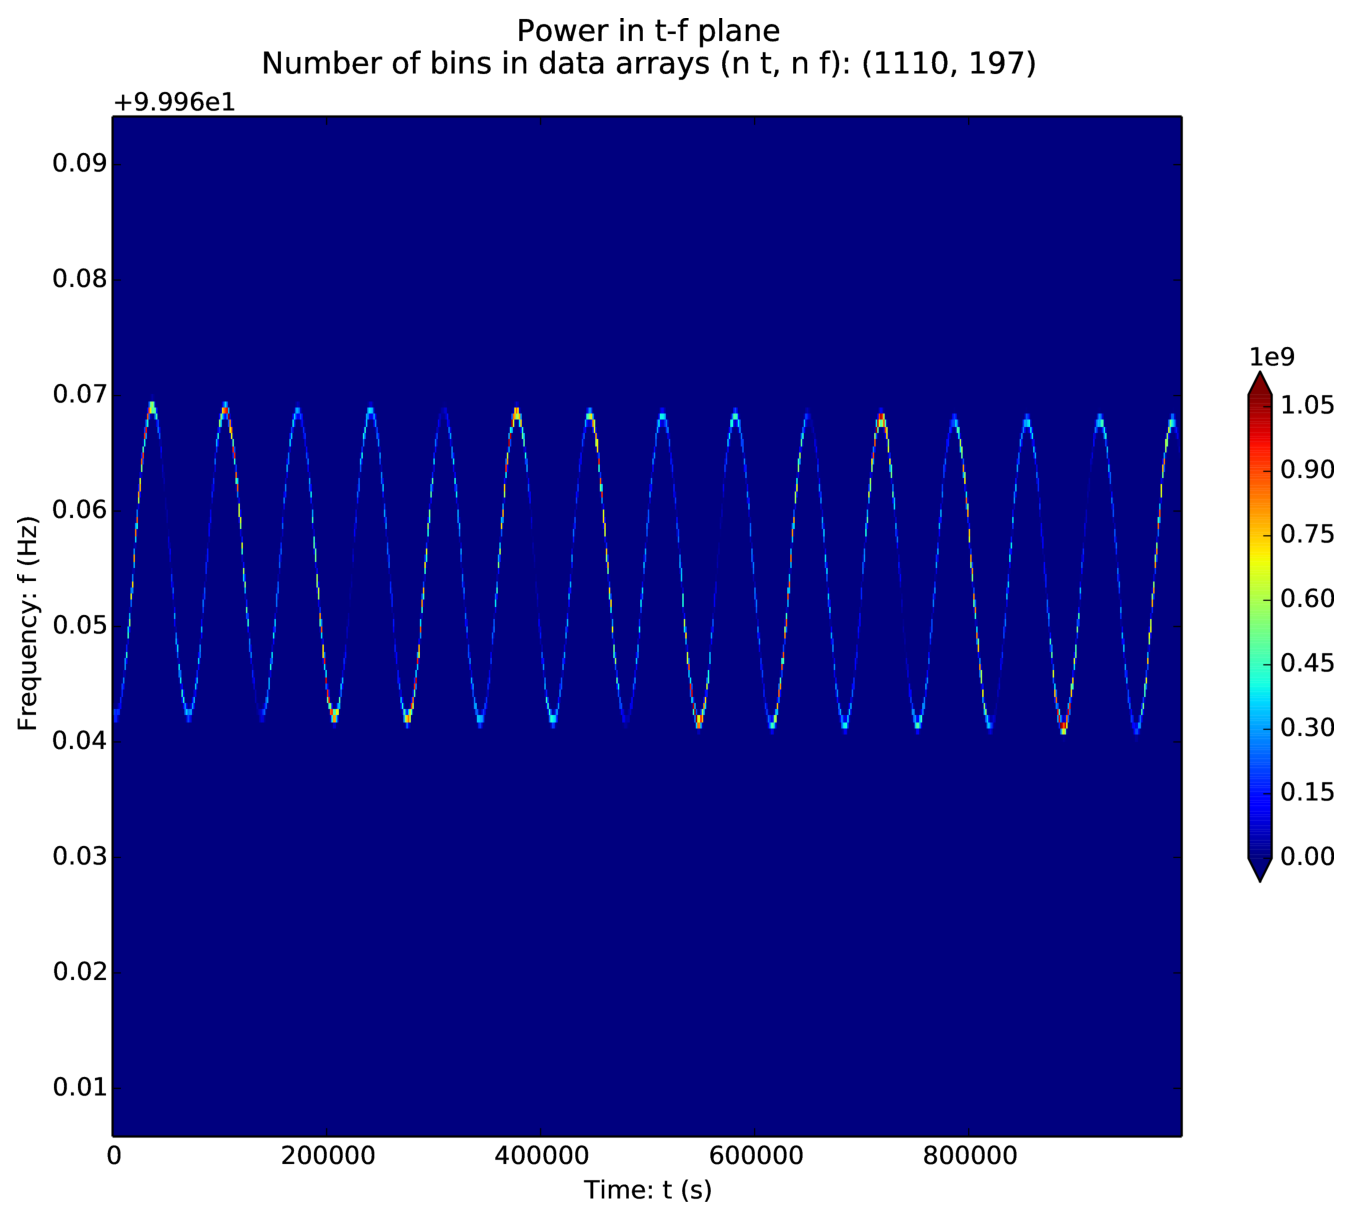
\includegraphics[trim=20 15 80 40, clip, keepaspectratio,height=0.35\paperheight]{plots/tfplane-4e21-on-4e24.eps}
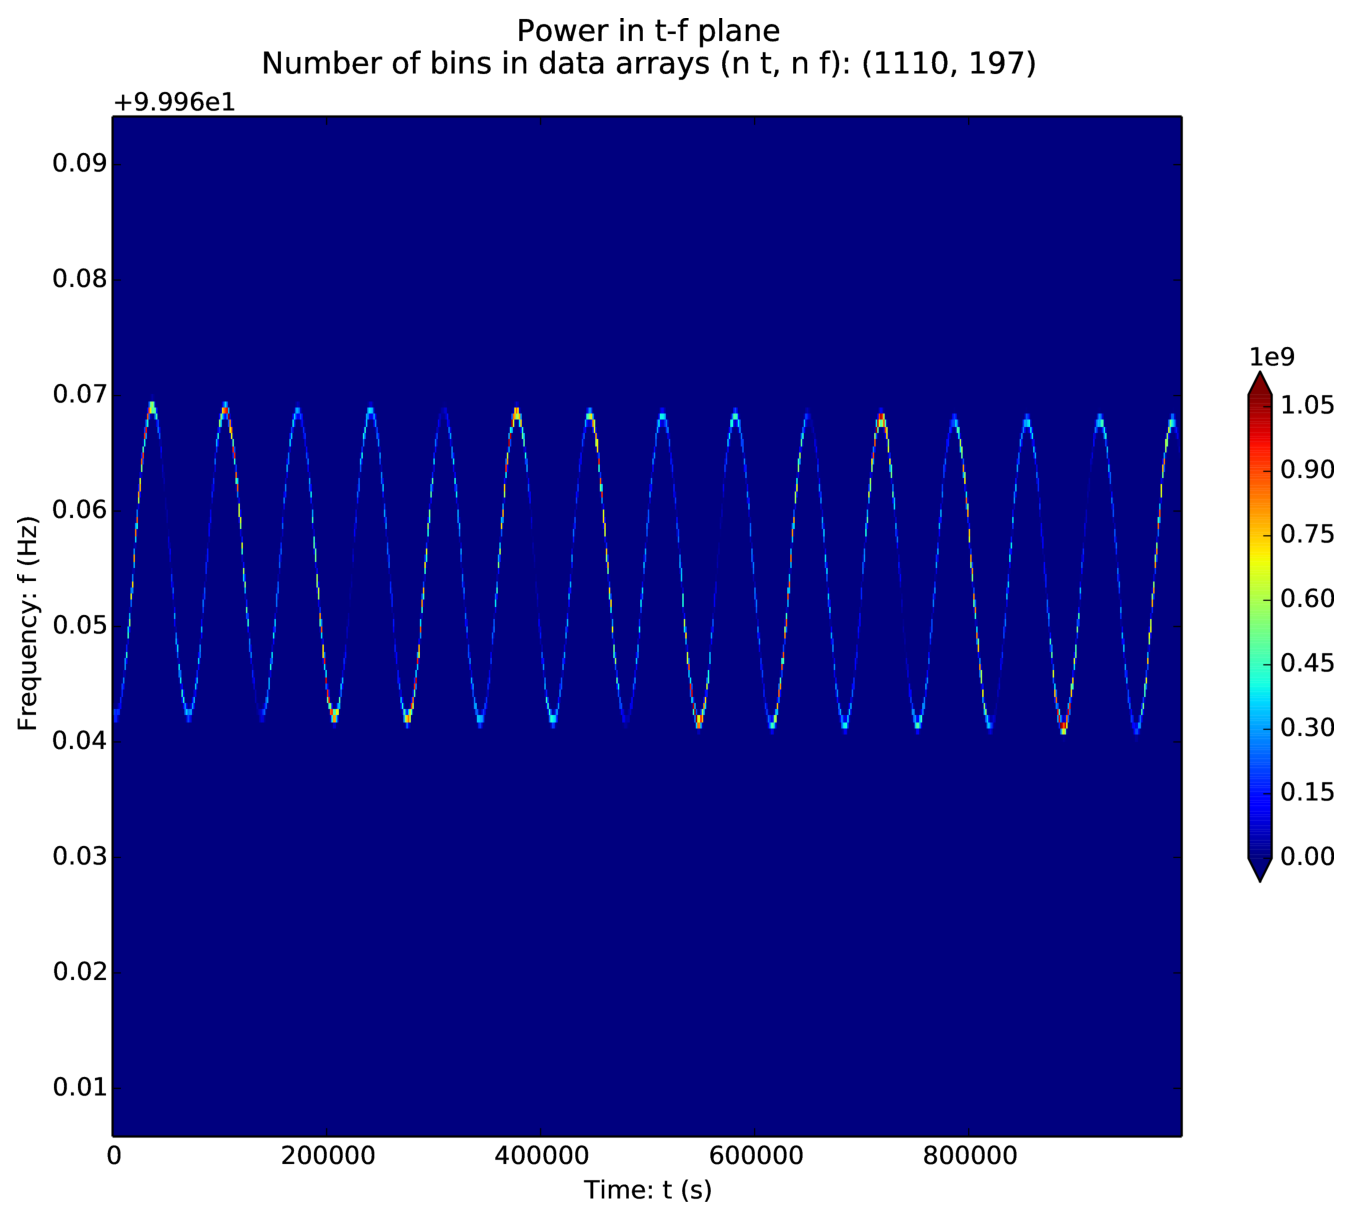
\includegraphics[keepaspectratio,height=0.35\paperheight]{plots/tfplane-4e21-on-4e24.eps}
\caption{By Doppler-shifting the frequencies into the solar system barycenter, TwoSpect makes this $f$ vs $t$ plane (pixel color indicates power). A simulated signal at 100.015 Hz with $P = 68023.8259$ s and $\mathrm{a} \sin i = 1.44$ modeling Sco X-1 is injected with $h_0 = 4\times 10^{-21}$ into $10^6$ s of Gaussian noise at $S^{1/2}_{h} = 4 \times 10^{-24}$ Hz$^{-1/2}$ (projected minimum Advanced LIGO noise).}
\label{tfplane-figure}
\end{center}
\end{figure}

\begin{figure}
\begin{center}
%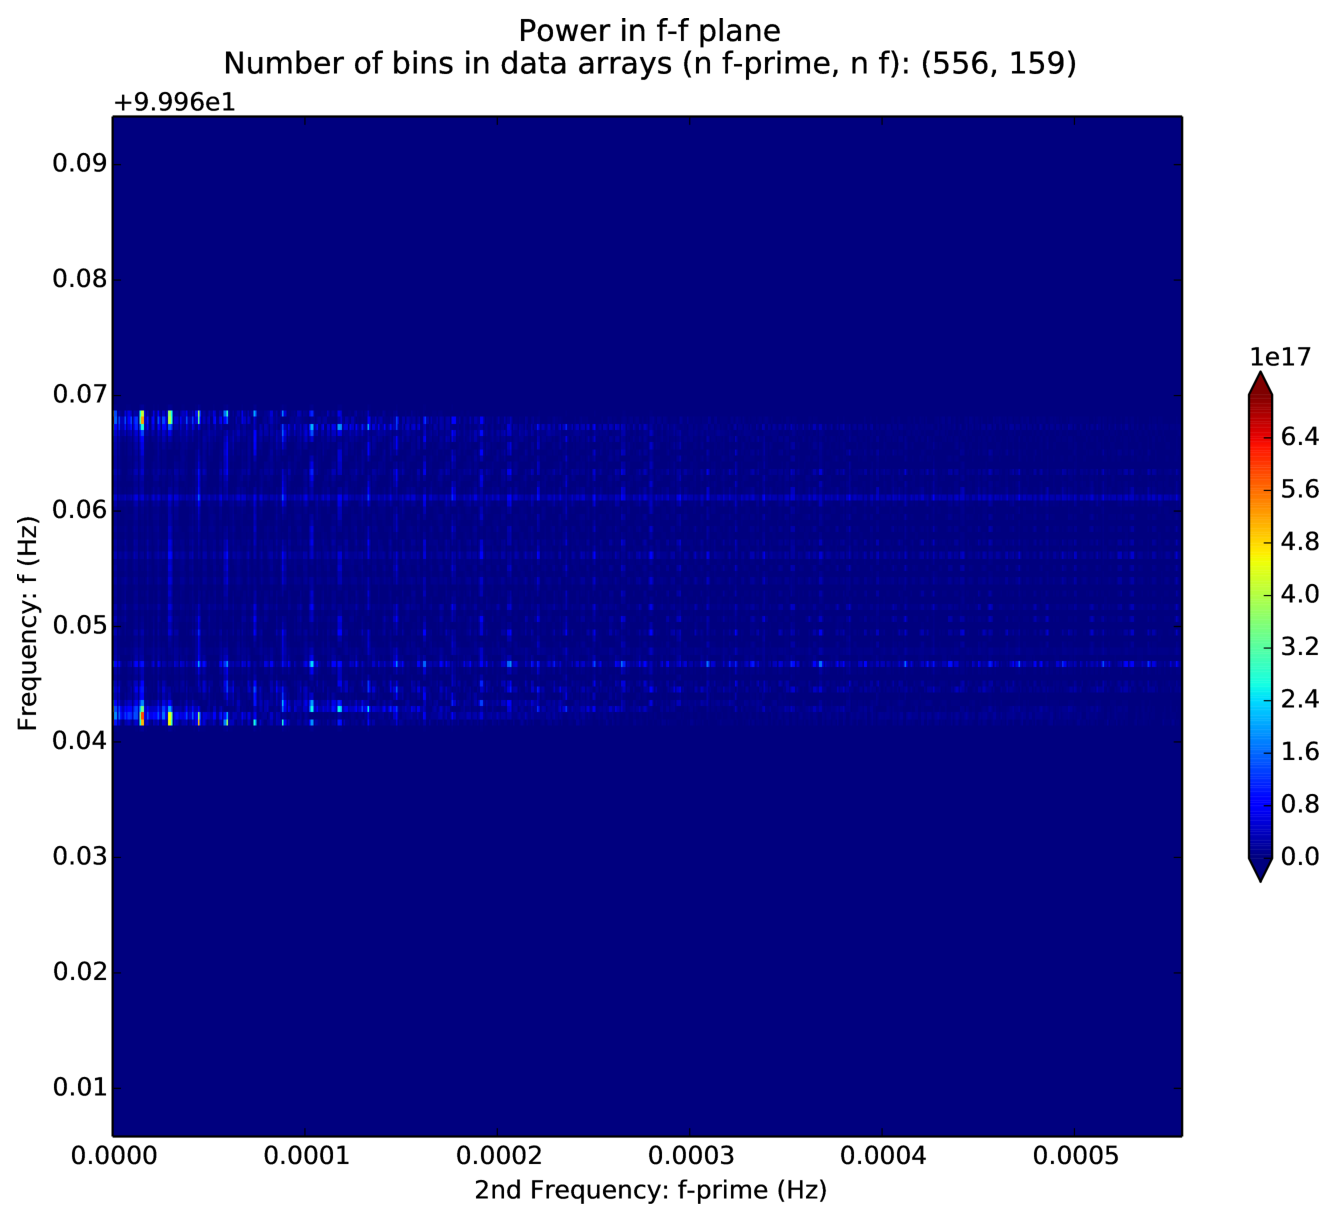
\includegraphics[trim=20 15 80 40, clip, keepaspectratio,height=0.35\paperheight]{plots/ffplane-4e21-on-4e24.eps}
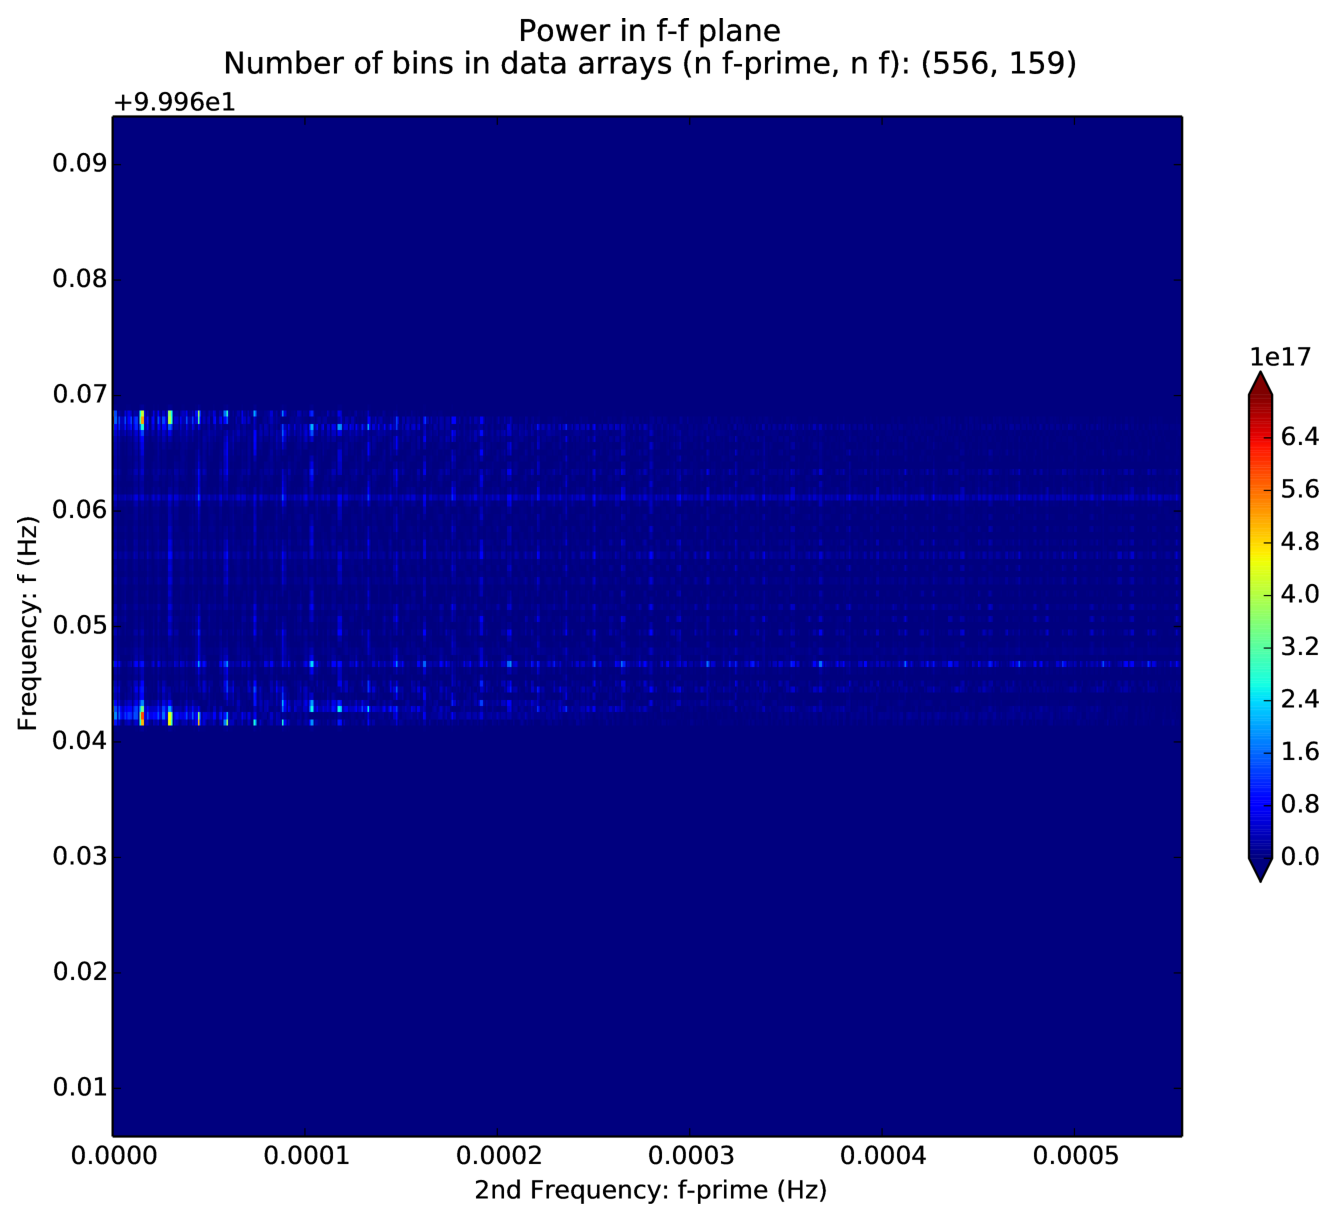
\includegraphics[keepaspectratio,height=0.35\paperheight]{plots/ffplane-4e21-on-4e24.eps}
\caption{Fourier-transforming along the time bins of each frequency row yields the $f$ vs $f'$ plane (pixel color indicates power). Templates are matched against pixels to compute the $R$ statistic. NOTE: the $x$-axis label is in fact \textit{bin number} and each value is the 2nd Fourier frequency in Hz times 1800 s.}
\label{ffplane-figure}
\end{center}
\end{figure}

%            \subsection{Inferring neutron stars with companions}
%            \label{inference}
 
Templates only vary for GW emission frequency $f$ and projected semi-major axis $a \sin i$, if orbital period $P$ and sky location are known.
%Projected semi-major axis manifests as a GW frequency modulation depth $\Delta f$~\cite{GoetzTwoSpectMethods2011},
%\begin{equation}
%\Delta f = \frac{2 \pi f (a \sin i)}{c P},
%\label{TwoSpect_mod_depth}
%\end{equation}
TwoSpect calculates an $R$ detection statistic~\cite{GoetzTwoSpectMethods2011} by taking the normed inner product of template weights $w_i$ with background $\lambda_i$-subtracted second-Fourier power $Z_i$ (Equation~\ref{TwoSpect_R_statistic}).

\noindent Define the inner product $<\vec{u}, \vec{v}>$, with norm squared $||\vec{u}||^2 \equiv <\vec{u}, \vec{u}>$ and projection $\mathit{proj}_{\vec{u}} \vec{v} \equiv ||\vec{u}||^{-2} <\vec{v}, \vec{u}> \vec{u}$:

\begin{eqnarray}
<\vec{u}, \vec{v}> \equiv \sum_{i=0}^{M-1} u_i v_i,\\
R = ||\vec{w}||^{-2} \cdot \left<\vec{w}, (\vec{Z} - \vec{\lambda})\right>,\\
\mathit{proj}_{\vec{w}} \left(\vec{Z} - \vec{\lambda} \right) = R \vec{w},
\label{TwoSpect_R_statistic_as_projection}
\end{eqnarray}

\noindent so $R$ is the scale of the projection of background-subtracted data onto template weights.
Although TwoSpect is not a matched filter, the definition of the $R$ statistic is analogous to the definition of a matched filter SNR, where templates are the filter coefficients and the noise covariance matrix is diagonal.

%$R$-statistic -- weighted sum of $\chi^2$ powers:
%searches for patterns in
%doubly Fourier-transformed data from binary's orbital modulation
%\emph{doubly Fourier-transformed:} $k$ frequency bins, time series
%$n$
%Short Fourier Transform series, along $n$, is FFT'd 

%\[
%R=\frac{\Sigma_{i=0}^{M-1}w(m_{i})[Z(m_{i})-\lambda(m_{i})]}{\Sigma_{i=0}^{M-1}[w(m_{i})]^{2}}
%\]

%\noindent for template weight $w$, spectral power $Z$,
%and background noise power $\lambda$,

As defined currently, the $R$ statistic 
(Figure~\ref{inj_R_statistic})
is not sensitive to orbital phase $T_\mathrm{asc}$; it is also insensitive to $\Phi_0$ and the reference time $T_\mathrm{ref}$ and robust against spin-wandering $\delta \Phi_\mathrm{spin-wander}$.
Single-template $p$-values (Figure~\ref{inj_log10p}) are extrapolated from $R$ values using the Davies' method, based on the characteristic function $\phi_R (u)$ of $R$~\cite{GoetzTwoSpectMethods2011}.
Up to a rescaling factor $\alpha_R$ corresponding to mean subtraction, this function is the product of the characteristic functions of the $\chi^2$-distributed weights, 

\begin{equation}
\phi_R(u) = \alpha_R \prod\limits_{i=1}^{M} \frac{1}{1 - \mathrm{i} u w'_i \lambda_i},
\end{equation}

\noindent where the primed weight $w'_i$ is

\begin{eqnarray}
w'_i = \frac{w_i}{\sum\limits_{j=0}^{M-1} w_j^2}.
%\alpha_R = \prod\limits_{i=1}^M \frac{1}{1 + \mathrm{i} w'_i }
\end{eqnarray}

\noindent Davies' method extrapolates the $p$-value from the Fourier transform of this characteristic function.
It breaks the integral over $u$ into steps indexed by $k_u = (u/\Delta_u - 1/2)$, of interval $\Delta_u$.
The number of steps, $K_u$, is numerically determined as needed for converegence.
The $p$-value is $P (R \geq R_0)$:

\begin{eqnarray}
P(R \geq R_0) &= 1 - \left(\frac{1}{2} \int_{-\infty}^{+\infty} \Im \left(\frac{\phi_R(u)e^{-\mathrm{i} u R_0}}{2 \pi u} \right) \mathrm{d}u \right),\\
  &= 1 - \left(\frac{1}{2} - \sum\limits_{k_u = 0}^{K_u} (\Pi_M S_k(R_0)) \right),
\end{eqnarray}
\begin{eqnarray}
\Pi_M = \prod\limits_{i=1}^{M-1} (1 + 4 u^2 \lambda_i^2)^{-1/2},\\
S_{k_u}  = \frac{1}{\pi \cdot (k_u+1/2)}\left(\sin \left[\sum_{i=0}^{M-1} \left( \arctan{(2 u w_i' \lambda_i)} \right) - u \cdot c(R_0)\right] \right),\\
c(R_0) =  R_0 + \sum\limits_{i=0}^{M-1} w_i' \lambda_i.
\end{eqnarray}

% From c(R_0) we should be easily able to read off \alpha_R, and I think it is
% indeed just a scale (like the \sum term after R_0 in C(R_0)).
% Point out that is where the data/background enters in, turning Prob
% into a simple scalar function of R_0,
% and then we calculate R_0 as a function of data in our experiment
% 
% Also, point out that the background is NOT slided (maybe point this out
% when <P_k>^n is introduced
%
% And then calculate the likelihood, either/both the data and of R
% 
% And then look up moment generating and characteristic functions
% to verify whether Gil-Pelaez is so obvious.
% -- answer: yes, it is, because we all agree
% that for pdf p(x) and characteristic \phi(t)
% p(x)  = \frac{1}{2\pi}\int e^{-itx} \phi(t) dt
% and we know integration is equivalent to dividing by 1/s in a Laplace
% transform, or, here, s = -i t (Characteristic function is a conjugated
% Fourier transform), so the cdf P(x) is
% P(x) = \frac{1}{2\pi}\int e^{-itx} \left(\frac{\phi(t)}{-it}\right) dt
% of course this integral is indefinite up to a constant, so
% Levy defined it as 
% P(b) - P(a) = \ldots \\
% \frac{1}{2\pi}\int (e^{-ita} - e^{-itb}) \left(\frac{\phi(t)}{-it}\right)
% 
% Oh, and check -- there is a factor of (1/2) or 2 in the 1 - i u \lambda w'
% denominator

\begin{figure}
\begin{center}
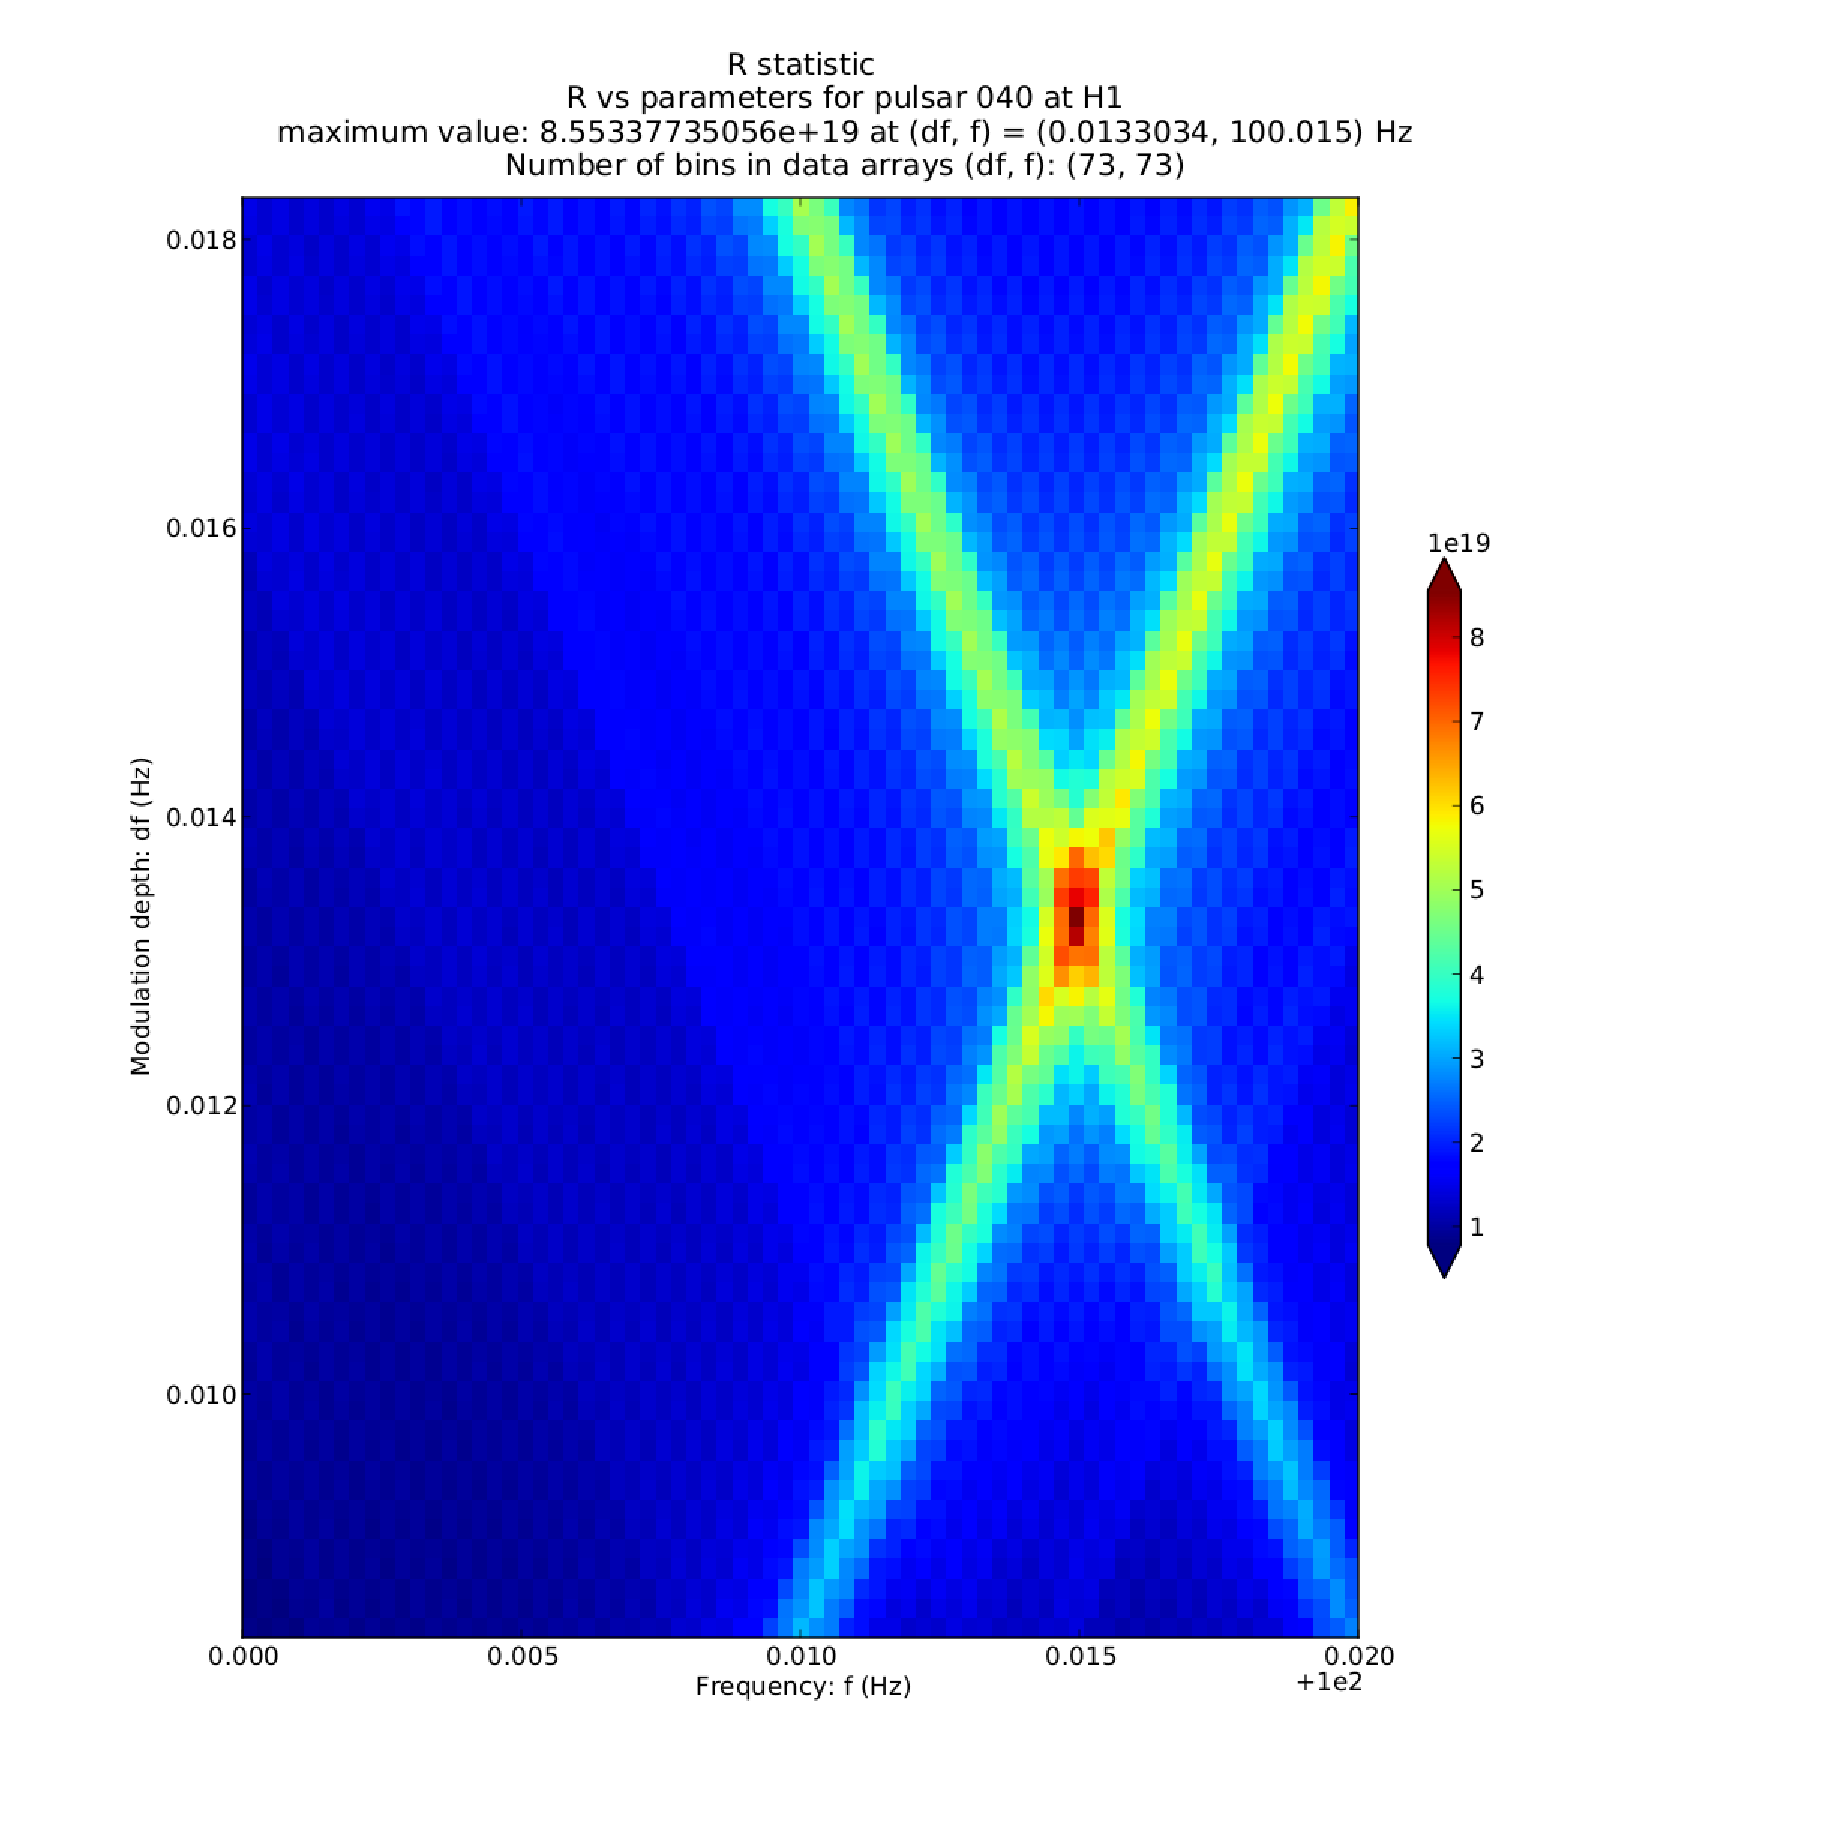
\includegraphics[trim=20 20 20 80, clip, keepaspectratio,height=0.55\paperheight]{plots/R-4e21-on-4e24.eps}
\caption{Signal templates applied to pixels in the $f$-$f'$ plane give $R$ statistics for a simulated pulsar 
%(note: not the same as pulsar $40$ in the Scorpius X-1 mock data challenge) 
at 100.015 Hz and $a \sin i = 1.44$ s. Resulting $R$ values are heatmap-plotted on the $\Delta f$ vs $f$ plane.}
\label{inj_R_statistic}
\end{center}
\end{figure}

\begin{figure}
\begin{center}
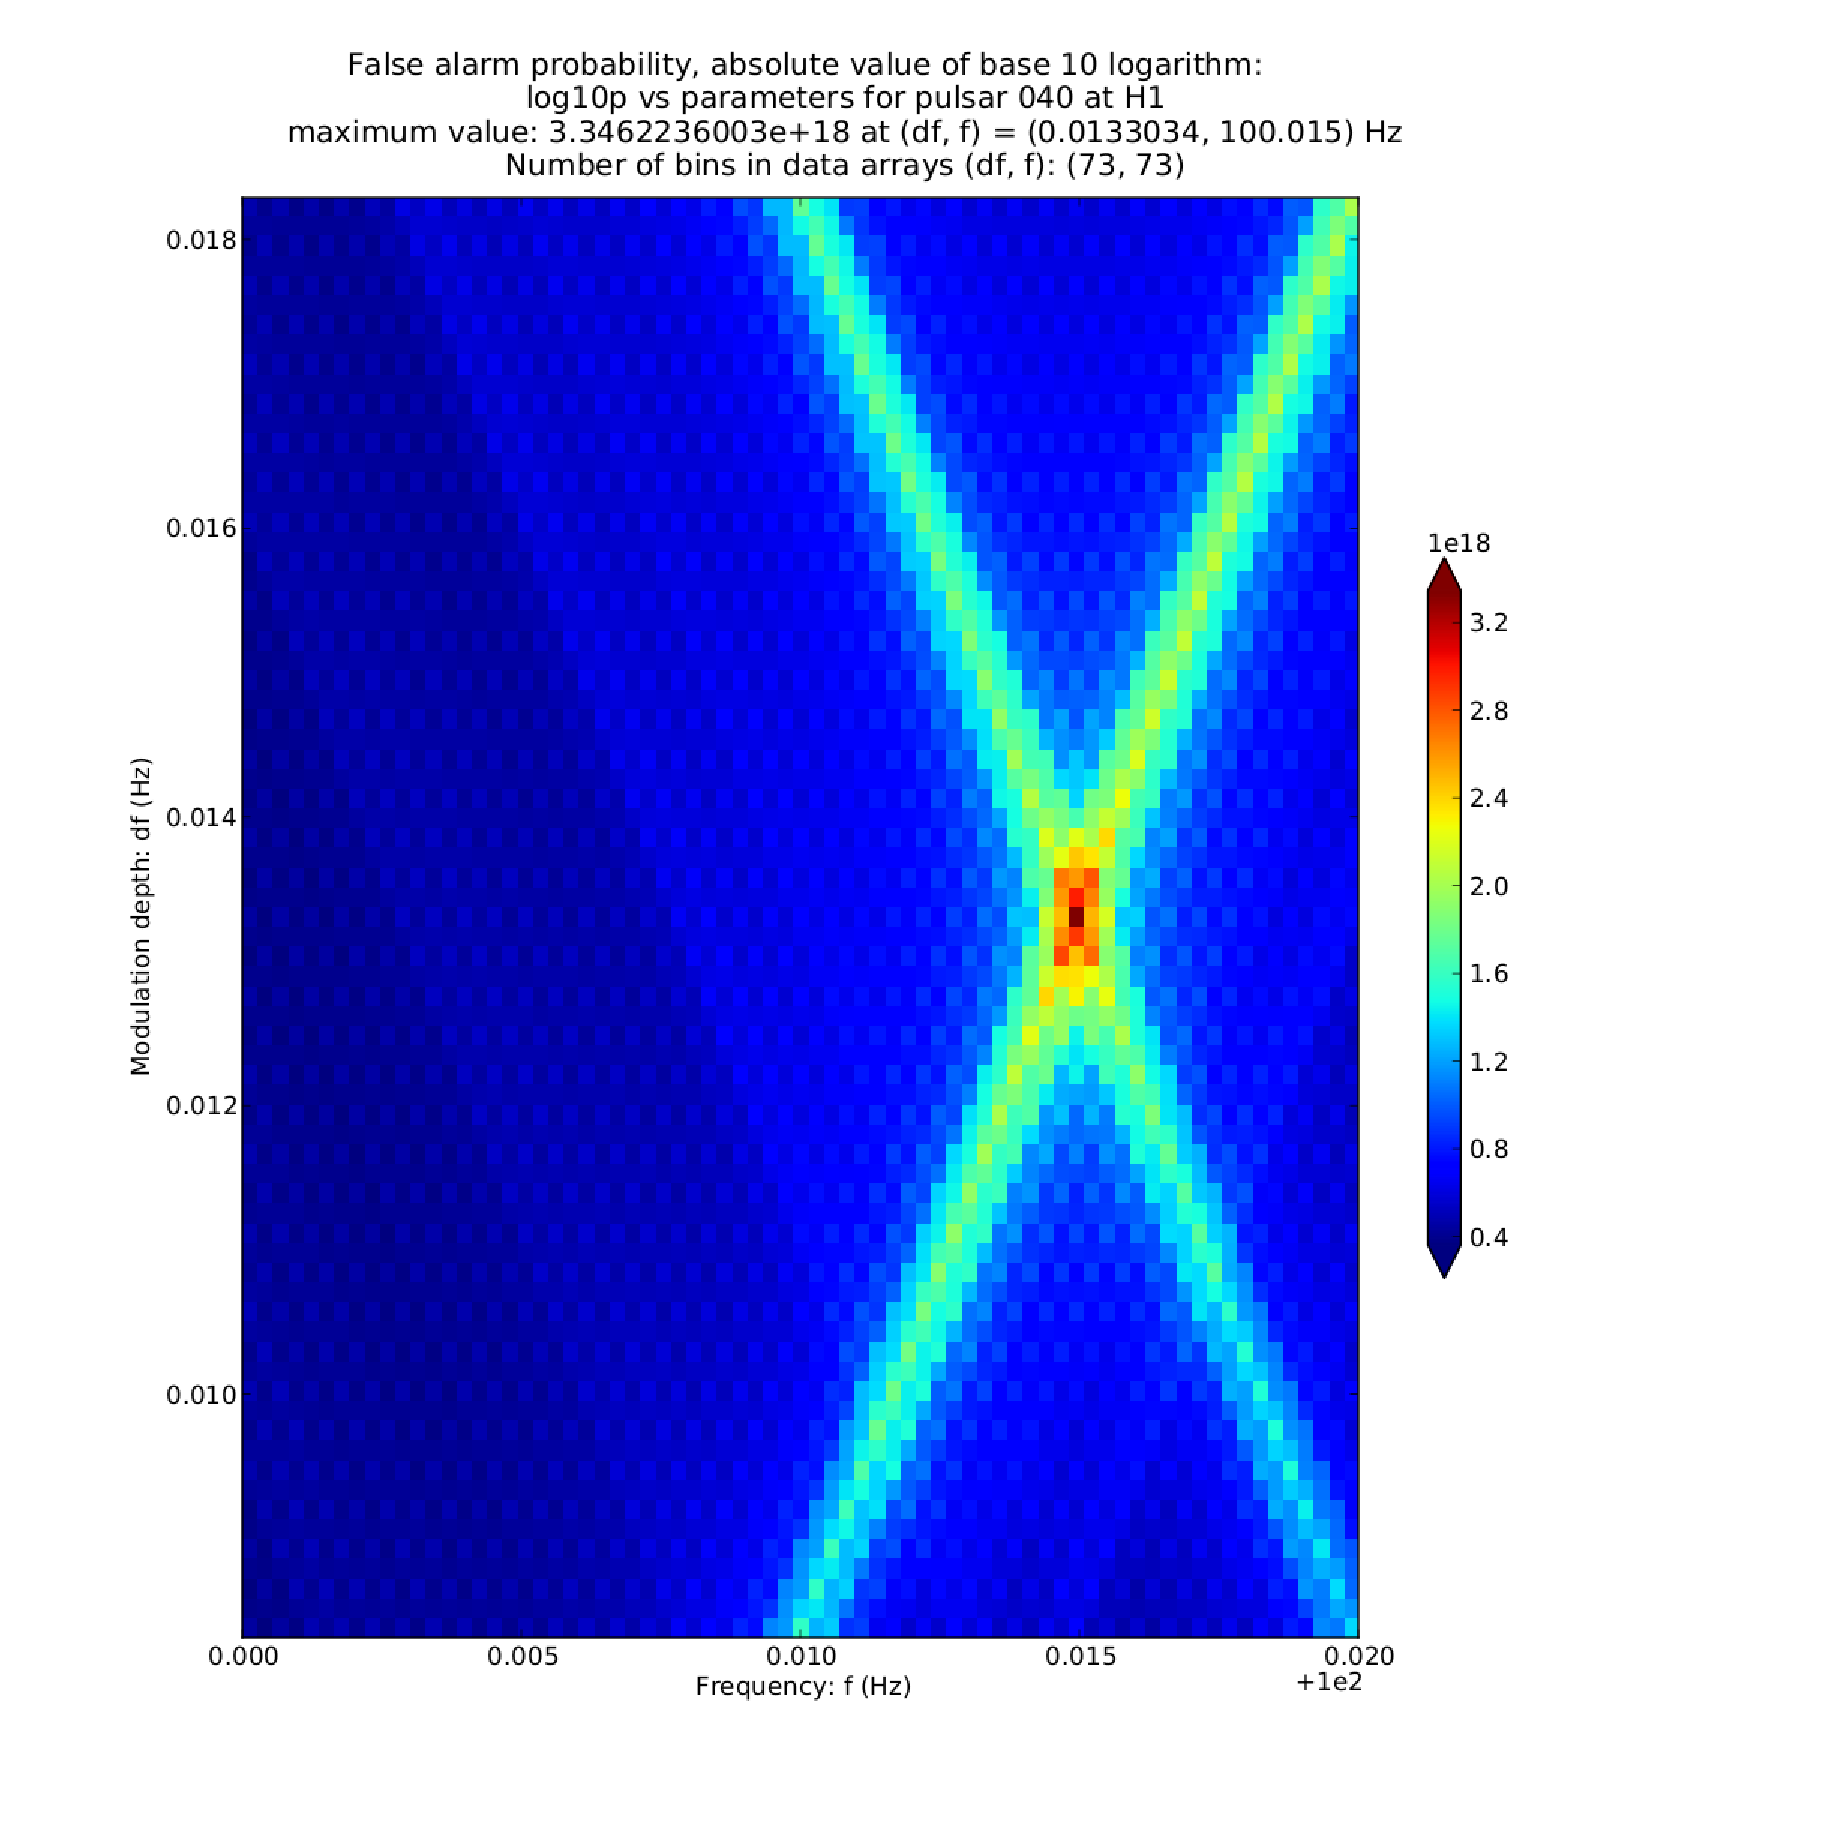
\includegraphics[trim=20 20 20 80, clip, keepaspectratio,height=0.55\paperheight]{plots/Prob-4e21-on-4e24.eps}
\caption{Davies' algorithm translates $R$ statistics into (single-template) $p$-values, plotted on the $\Delta f$ vs $f$ plane.}
\label{inj_log10p}
\end{center}
\end{figure}

\subsection{Template spacing and search metrics}

Searches are conducted by testing a recorded data set using templates corresponding to a putative GW signal.
Many templates are needed, depending on the scale of the search~\cite{GoetzTwoSpectMethods2011}, to cover the range of possible parameters $\theta$.
In the all-sky search, parameters include orbital period $P$ and sky location $(\alpha, \delta)$, but the directed search described herein can be used when these are known, so the parameter space is restricted to frequency $f$ and projected semi-major axis $a \sin i$.
The parameter space grid must be sampled densely enough to constrain $R$-statistic mismatch $\mu \leq 0.2$.
Mismatch is defined by the fractional difference between the $R$ statistic at the true parameters of the signal, $R(\theta_{GW})$, from the maximum $R(\theta)$ obtained; the statistic is designed so that idealy $R(\theta_{GW}) \geq R(\theta)$ for all $\theta$, assuming one signal is present.
Prior simulations have shown that, when $P$ and $(\alpha,\delta)$ are fixed, the $f$ and $a \sin i$ grids are uniform.
Frequency $f$ spacing of $1/2T_\mathrm{SFT}$ is sufficient, and $a \sin i$ is chosen such that modulation depth $\Delta f_\mathrm{obs}$ is spaced at $1/4T_\mathrm{SFT}$.
For a fuller analysis, one can calculate the statistical mismatch metric~\cite{Brady1998}, $g_{ij}$.
Fixed grid spacing corresponds to a flat mismatch metric.



\end{document}
